% Options for packages loaded elsewhere
\PassOptionsToPackage{unicode}{hyperref}
\PassOptionsToPackage{hyphens}{url}
\PassOptionsToPackage{dvipsnames,svgnames,x11names}{xcolor}
%
\documentclass[
  letterpaper,
  DIV=11,
  numbers=noendperiod]{scrreprt}

\usepackage{amsmath,amssymb}
\usepackage{iftex}
\ifPDFTeX
  \usepackage[T1]{fontenc}
  \usepackage[utf8]{inputenc}
  \usepackage{textcomp} % provide euro and other symbols
\else % if luatex or xetex
  \usepackage{unicode-math}
  \defaultfontfeatures{Scale=MatchLowercase}
  \defaultfontfeatures[\rmfamily]{Ligatures=TeX,Scale=1}
\fi
\usepackage{lmodern}
\ifPDFTeX\else  
    % xetex/luatex font selection
\fi
% Use upquote if available, for straight quotes in verbatim environments
\IfFileExists{upquote.sty}{\usepackage{upquote}}{}
\IfFileExists{microtype.sty}{% use microtype if available
  \usepackage[]{microtype}
  \UseMicrotypeSet[protrusion]{basicmath} % disable protrusion for tt fonts
}{}
\makeatletter
\@ifundefined{KOMAClassName}{% if non-KOMA class
  \IfFileExists{parskip.sty}{%
    \usepackage{parskip}
  }{% else
    \setlength{\parindent}{0pt}
    \setlength{\parskip}{6pt plus 2pt minus 1pt}}
}{% if KOMA class
  \KOMAoptions{parskip=half}}
\makeatother
\usepackage{xcolor}
\setlength{\emergencystretch}{3em} % prevent overfull lines
\setcounter{secnumdepth}{5}
% Make \paragraph and \subparagraph free-standing
\makeatletter
\ifx\paragraph\undefined\else
  \let\oldparagraph\paragraph
  \renewcommand{\paragraph}{
    \@ifstar
      \xxxParagraphStar
      \xxxParagraphNoStar
  }
  \newcommand{\xxxParagraphStar}[1]{\oldparagraph*{#1}\mbox{}}
  \newcommand{\xxxParagraphNoStar}[1]{\oldparagraph{#1}\mbox{}}
\fi
\ifx\subparagraph\undefined\else
  \let\oldsubparagraph\subparagraph
  \renewcommand{\subparagraph}{
    \@ifstar
      \xxxSubParagraphStar
      \xxxSubParagraphNoStar
  }
  \newcommand{\xxxSubParagraphStar}[1]{\oldsubparagraph*{#1}\mbox{}}
  \newcommand{\xxxSubParagraphNoStar}[1]{\oldsubparagraph{#1}\mbox{}}
\fi
\makeatother

\usepackage{color}
\usepackage{fancyvrb}
\newcommand{\VerbBar}{|}
\newcommand{\VERB}{\Verb[commandchars=\\\{\}]}
\DefineVerbatimEnvironment{Highlighting}{Verbatim}{commandchars=\\\{\}}
% Add ',fontsize=\small' for more characters per line
\usepackage{framed}
\definecolor{shadecolor}{RGB}{241,243,245}
\newenvironment{Shaded}{\begin{snugshade}}{\end{snugshade}}
\newcommand{\AlertTok}[1]{\textcolor[rgb]{0.68,0.00,0.00}{#1}}
\newcommand{\AnnotationTok}[1]{\textcolor[rgb]{0.37,0.37,0.37}{#1}}
\newcommand{\AttributeTok}[1]{\textcolor[rgb]{0.40,0.45,0.13}{#1}}
\newcommand{\BaseNTok}[1]{\textcolor[rgb]{0.68,0.00,0.00}{#1}}
\newcommand{\BuiltInTok}[1]{\textcolor[rgb]{0.00,0.23,0.31}{#1}}
\newcommand{\CharTok}[1]{\textcolor[rgb]{0.13,0.47,0.30}{#1}}
\newcommand{\CommentTok}[1]{\textcolor[rgb]{0.37,0.37,0.37}{#1}}
\newcommand{\CommentVarTok}[1]{\textcolor[rgb]{0.37,0.37,0.37}{\textit{#1}}}
\newcommand{\ConstantTok}[1]{\textcolor[rgb]{0.56,0.35,0.01}{#1}}
\newcommand{\ControlFlowTok}[1]{\textcolor[rgb]{0.00,0.23,0.31}{\textbf{#1}}}
\newcommand{\DataTypeTok}[1]{\textcolor[rgb]{0.68,0.00,0.00}{#1}}
\newcommand{\DecValTok}[1]{\textcolor[rgb]{0.68,0.00,0.00}{#1}}
\newcommand{\DocumentationTok}[1]{\textcolor[rgb]{0.37,0.37,0.37}{\textit{#1}}}
\newcommand{\ErrorTok}[1]{\textcolor[rgb]{0.68,0.00,0.00}{#1}}
\newcommand{\ExtensionTok}[1]{\textcolor[rgb]{0.00,0.23,0.31}{#1}}
\newcommand{\FloatTok}[1]{\textcolor[rgb]{0.68,0.00,0.00}{#1}}
\newcommand{\FunctionTok}[1]{\textcolor[rgb]{0.28,0.35,0.67}{#1}}
\newcommand{\ImportTok}[1]{\textcolor[rgb]{0.00,0.46,0.62}{#1}}
\newcommand{\InformationTok}[1]{\textcolor[rgb]{0.37,0.37,0.37}{#1}}
\newcommand{\KeywordTok}[1]{\textcolor[rgb]{0.00,0.23,0.31}{\textbf{#1}}}
\newcommand{\NormalTok}[1]{\textcolor[rgb]{0.00,0.23,0.31}{#1}}
\newcommand{\OperatorTok}[1]{\textcolor[rgb]{0.37,0.37,0.37}{#1}}
\newcommand{\OtherTok}[1]{\textcolor[rgb]{0.00,0.23,0.31}{#1}}
\newcommand{\PreprocessorTok}[1]{\textcolor[rgb]{0.68,0.00,0.00}{#1}}
\newcommand{\RegionMarkerTok}[1]{\textcolor[rgb]{0.00,0.23,0.31}{#1}}
\newcommand{\SpecialCharTok}[1]{\textcolor[rgb]{0.37,0.37,0.37}{#1}}
\newcommand{\SpecialStringTok}[1]{\textcolor[rgb]{0.13,0.47,0.30}{#1}}
\newcommand{\StringTok}[1]{\textcolor[rgb]{0.13,0.47,0.30}{#1}}
\newcommand{\VariableTok}[1]{\textcolor[rgb]{0.07,0.07,0.07}{#1}}
\newcommand{\VerbatimStringTok}[1]{\textcolor[rgb]{0.13,0.47,0.30}{#1}}
\newcommand{\WarningTok}[1]{\textcolor[rgb]{0.37,0.37,0.37}{\textit{#1}}}

\providecommand{\tightlist}{%
  \setlength{\itemsep}{0pt}\setlength{\parskip}{0pt}}\usepackage{longtable,booktabs,array}
\usepackage{calc} % for calculating minipage widths
% Correct order of tables after \paragraph or \subparagraph
\usepackage{etoolbox}
\makeatletter
\patchcmd\longtable{\par}{\if@noskipsec\mbox{}\fi\par}{}{}
\makeatother
% Allow footnotes in longtable head/foot
\IfFileExists{footnotehyper.sty}{\usepackage{footnotehyper}}{\usepackage{footnote}}
\makesavenoteenv{longtable}
\usepackage{graphicx}
\makeatletter
\def\maxwidth{\ifdim\Gin@nat@width>\linewidth\linewidth\else\Gin@nat@width\fi}
\def\maxheight{\ifdim\Gin@nat@height>\textheight\textheight\else\Gin@nat@height\fi}
\makeatother
% Scale images if necessary, so that they will not overflow the page
% margins by default, and it is still possible to overwrite the defaults
% using explicit options in \includegraphics[width, height, ...]{}
\setkeys{Gin}{width=\maxwidth,height=\maxheight,keepaspectratio}
% Set default figure placement to htbp
\makeatletter
\def\fps@figure{htbp}
\makeatother
% definitions for citeproc citations
\NewDocumentCommand\citeproctext{}{}
\NewDocumentCommand\citeproc{mm}{%
  \begingroup\def\citeproctext{#2}\cite{#1}\endgroup}
\makeatletter
 % allow citations to break across lines
 \let\@cite@ofmt\@firstofone
 % avoid brackets around text for \cite:
 \def\@biblabel#1{}
 \def\@cite#1#2{{#1\if@tempswa , #2\fi}}
\makeatother
\newlength{\cslhangindent}
\setlength{\cslhangindent}{1.5em}
\newlength{\csllabelwidth}
\setlength{\csllabelwidth}{3em}
\newenvironment{CSLReferences}[2] % #1 hanging-indent, #2 entry-spacing
 {\begin{list}{}{%
  \setlength{\itemindent}{0pt}
  \setlength{\leftmargin}{0pt}
  \setlength{\parsep}{0pt}
  % turn on hanging indent if param 1 is 1
  \ifodd #1
   \setlength{\leftmargin}{\cslhangindent}
   \setlength{\itemindent}{-1\cslhangindent}
  \fi
  % set entry spacing
  \setlength{\itemsep}{#2\baselineskip}}}
 {\end{list}}
\usepackage{calc}
\newcommand{\CSLBlock}[1]{\hfill\break\parbox[t]{\linewidth}{\strut\ignorespaces#1\strut}}
\newcommand{\CSLLeftMargin}[1]{\parbox[t]{\csllabelwidth}{\strut#1\strut}}
\newcommand{\CSLRightInline}[1]{\parbox[t]{\linewidth - \csllabelwidth}{\strut#1\strut}}
\newcommand{\CSLIndent}[1]{\hspace{\cslhangindent}#1}

\KOMAoption{captions}{tableheading}
\makeatletter
\@ifpackageloaded{tcolorbox}{}{\usepackage[skins,breakable]{tcolorbox}}
\@ifpackageloaded{fontawesome5}{}{\usepackage{fontawesome5}}
\definecolor{quarto-callout-color}{HTML}{909090}
\definecolor{quarto-callout-note-color}{HTML}{0758E5}
\definecolor{quarto-callout-important-color}{HTML}{CC1914}
\definecolor{quarto-callout-warning-color}{HTML}{EB9113}
\definecolor{quarto-callout-tip-color}{HTML}{00A047}
\definecolor{quarto-callout-caution-color}{HTML}{FC5300}
\definecolor{quarto-callout-color-frame}{HTML}{acacac}
\definecolor{quarto-callout-note-color-frame}{HTML}{4582ec}
\definecolor{quarto-callout-important-color-frame}{HTML}{d9534f}
\definecolor{quarto-callout-warning-color-frame}{HTML}{f0ad4e}
\definecolor{quarto-callout-tip-color-frame}{HTML}{02b875}
\definecolor{quarto-callout-caution-color-frame}{HTML}{fd7e14}
\makeatother
\makeatletter
\@ifpackageloaded{bookmark}{}{\usepackage{bookmark}}
\makeatother
\makeatletter
\@ifpackageloaded{caption}{}{\usepackage{caption}}
\AtBeginDocument{%
\ifdefined\contentsname
  \renewcommand*\contentsname{Table of contents}
\else
  \newcommand\contentsname{Table of contents}
\fi
\ifdefined\listfigurename
  \renewcommand*\listfigurename{List of Figures}
\else
  \newcommand\listfigurename{List of Figures}
\fi
\ifdefined\listtablename
  \renewcommand*\listtablename{List of Tables}
\else
  \newcommand\listtablename{List of Tables}
\fi
\ifdefined\figurename
  \renewcommand*\figurename{Figure}
\else
  \newcommand\figurename{Figure}
\fi
\ifdefined\tablename
  \renewcommand*\tablename{Table}
\else
  \newcommand\tablename{Table}
\fi
}
\@ifpackageloaded{float}{}{\usepackage{float}}
\floatstyle{ruled}
\@ifundefined{c@chapter}{\newfloat{codelisting}{h}{lop}}{\newfloat{codelisting}{h}{lop}[chapter]}
\floatname{codelisting}{Listing}
\newcommand*\listoflistings{\listof{codelisting}{List of Listings}}
\makeatother
\makeatletter
\makeatother
\makeatletter
\@ifpackageloaded{caption}{}{\usepackage{caption}}
\@ifpackageloaded{subcaption}{}{\usepackage{subcaption}}
\makeatother
\makeatletter
\@ifpackageloaded{fontawesome5}{}{\usepackage{fontawesome5}}
\makeatother
\ifLuaTeX
  \usepackage{selnolig}  % disable illegal ligatures
\fi
\usepackage{bookmark}

\IfFileExists{xurl.sty}{\usepackage{xurl}}{} % add URL line breaks if available
\urlstyle{same} % disable monospaced font for URLs
\hypersetup{
  pdftitle={Test Quarto Book},
  pdfauthor={Brad Cannell},
  colorlinks=true,
  linkcolor={blue},
  filecolor={Maroon},
  citecolor={Blue},
  urlcolor={Blue},
  pdfcreator={LaTeX via pandoc}}

\title{Test Quarto Book}
\author{Brad Cannell}
\date{2025-01-23}

\begin{document}
\maketitle

\renewcommand*\contentsname{Table of contents}
{
\hypersetup{linkcolor=}
\setcounter{tocdepth}{2}
\tableofcontents
}
\bookmarksetup{startatroot}

\chapter*{Preface}\label{preface}
\addcontentsline{toc}{chapter}{Preface}

\markboth{Preface}{Preface}

This is my first Quarto book. For now, I'm just using it for some
experimentation. Eventually, I will probably want to add all of this to
a GitHub repository. Right now, Olivia is in class and I'm content with
just experimenting a little bit.

This is \textbf{not} my new R Notes book; although, I may move R Notes
over to Quarto at some point. This is purely just a sandbox for playing
with Quarto books.

\section*{Useful websites:}\label{useful-websites}
\addcontentsline{toc}{section}{Useful websites:}

\markright{Useful websites:}

\begin{itemize}
\tightlist
\item
  \href{https://quarto.org/docs/books/}{Quarto book documentation}
\end{itemize}

\section*{Rendering}\label{rendering}
\addcontentsline{toc}{section}{Rendering}

\markright{Rendering}

You can render the files by clicking the Render button in RStudio. To
render the HTML and PDF files at the same time, type
\texttt{quarto\ render} into the terminal. You can also render Quarto
files with a native R code chunk.

\begin{itemize}
\item
  The input argument: The input file or project directory to be rendered
  (defaults to rendering the project in the current working directory).
\item
  The output\_format argument: Target output format (defaults to
  ``html''). The option ``all'' will render all formats defined within
  the file or project.
\end{itemize}

\begin{Shaded}
\begin{Highlighting}[]
\InformationTok{\textasciigrave{}\textasciigrave{}\textasciigrave{}\{r\}}
\InformationTok{\#| Render with R}
\InformationTok{\#| eval: false}
\InformationTok{quarto::quarto\_render(output\_format = "all")}
\InformationTok{\textasciigrave{}\textasciigrave{}\textasciigrave{}}
\end{Highlighting}
\end{Shaded}

\section*{Publishing to GitHub pages}\label{publishing-to-github-pages}
\addcontentsline{toc}{section}{Publishing to GitHub pages}

\markright{Publishing to GitHub pages}

\href{https://quarto.org/docs/publishing/github-pages.html}{This article
is great}.

\begin{itemize}
\tightlist
\item
  Make sure you are on the main branch.
\item
  After rendering (see above), make sure to save and \textbf{commit}
  your changes to GitHub.
\item
  Type \texttt{quarto\ publish\ gh-pages} in the terminal.
\end{itemize}

\part{Book Options}

This part of the book contains qmd files pertaining to book options. I'm
mostly creating this file to demonstrate how the (optional) book part
qmd files work.

\chapter{Book Options}\label{sec-book-options}

A collection of notes on Quarto book options.

\begin{itemize}
\item
  \href{https://quarto.org/docs/reference/projects/books.html}{Link to
  list of book options}
\item
  How do you add a cover image? Look at
  \href{https://github.com/hadley/r4ds/}{r4ds}.

  \begin{itemize}
  \tightlist
  \item
    \texttt{cover-image:\ cover.jpg}
  \end{itemize}
\item
  How do you add last date rendered to the \texttt{\_quarto.yml} file?
  ``r Sys.Date()'' doesn't seem to work.

  \begin{itemize}
  \tightlist
  \item
    \href{https://biostats-r.github.io/biostats/quarto/03-elements-quarto-document.html}{Use
    the keyword today}
  \end{itemize}
\item
  Can I add links to GitHub and/or social media?

  \begin{itemize}
  \tightlist
  \item
    Still need an answer here.
  \end{itemize}
\item
  Can I add links to the GitHub repo containing the books files?

  \begin{itemize}
  \tightlist
  \item
    Yes. See
    https://quarto.org/docs/books/book-output.html\#sidebar-tools
  \end{itemize}
\item
  How do I add a favicon?

  \begin{itemize}
  \tightlist
  \item
    \texttt{favicon:\ cover.jpg}
  \end{itemize}
\item
  How do I add Google analytics?

  \begin{itemize}
  \tightlist
  \item
    Still need an answer here.
  \end{itemize}
\item
  Can I add a Google analytics badge to my GitHub README?

  \begin{itemize}
  \tightlist
  \item
    Still need an answer here.
  \end{itemize}
\item
  How do I preview the book in my web browser instead of RStudio's
  Viewer pane?

  \begin{itemize}
  \tightlist
  \item
    Just click the little gear icon next to the \texttt{Render} button
    in RStudio. Select \texttt{Preview\ in\ Window}.
  \end{itemize}
\end{itemize}

\chapter{Other little things}\label{other}

\section{Pros and cons}\label{pros-and-cons}

Some of the things I like about working with Quarto (as opposed to
bookdown) so far

\begin{itemize}
\item
  A preview of the book renders automatically.
\item
  I can easily render only one chapter by opening that chapter's qmd
  file and clicking the Render button.
\end{itemize}

\part{Authoring}

\chapter{Adding call out boxes}\label{adding-call-out-boxes}

In R4Epi, we sometimes add special boxes for side notes and warnings.
How do we add those into qmd books?

What do those boxes look like when we render the book to pdf format?

Does Quarto have some built-in boxes? It looks like it might?

\begin{itemize}
\tightlist
\item
  How do you add the call out boxes (i.e., important, etc.)?

  \begin{itemize}
  \tightlist
  \item
    See \href{https://quarto.org/docs/authoring/callouts.html}{Quarto
    documentation on callout blocks}
  \end{itemize}
\end{itemize}

\begin{Shaded}
\begin{Highlighting}[]
\NormalTok{::: callout{-}note}
\NormalTok{Note that there are five types of callouts, including: }\InformationTok{\textasciigrave{}note\textasciigrave{}}\NormalTok{, }\InformationTok{\textasciigrave{}tip\textasciigrave{}}\NormalTok{, }\InformationTok{\textasciigrave{}warning\textasciigrave{}}\NormalTok{, }\InformationTok{\textasciigrave{}caution\textasciigrave{}}\NormalTok{, and }\InformationTok{\textasciigrave{}important\textasciigrave{}}\NormalTok{.}
\NormalTok{:::}
\end{Highlighting}
\end{Shaded}

\begin{tcolorbox}[enhanced jigsaw, breakable, title=\textcolor{quarto-callout-note-color}{\faInfo}\hspace{0.5em}{Note}, bottomrule=.15mm, coltitle=black, left=2mm, colbacktitle=quarto-callout-note-color!10!white, colback=white, toprule=.15mm, leftrule=.75mm, arc=.35mm, colframe=quarto-callout-note-color-frame, bottomtitle=1mm, toptitle=1mm, opacityback=0, titlerule=0mm, opacitybacktitle=0.6, rightrule=.15mm]

Note that there are five types of callouts, including: \texttt{note},
\texttt{tip}, \texttt{warning}, \texttt{caution}, and
\texttt{important}.

\end{tcolorbox}

\begin{Shaded}
\begin{Highlighting}[]
\NormalTok{::: callout{-}warning}
\NormalTok{Callouts provide a simple way to attract attention, for example, to this warning.}
\NormalTok{:::}
\end{Highlighting}
\end{Shaded}

\begin{tcolorbox}[enhanced jigsaw, breakable, title=\textcolor{quarto-callout-warning-color}{\faExclamationTriangle}\hspace{0.5em}{Warning}, bottomrule=.15mm, coltitle=black, left=2mm, colbacktitle=quarto-callout-warning-color!10!white, colback=white, toprule=.15mm, leftrule=.75mm, arc=.35mm, colframe=quarto-callout-warning-color-frame, bottomtitle=1mm, toptitle=1mm, opacityback=0, titlerule=0mm, opacitybacktitle=0.6, rightrule=.15mm]

Callouts provide a simple way to attract attention, for example, to this
warning.

\end{tcolorbox}

\begin{Shaded}
\begin{Highlighting}[]
\NormalTok{::: callout{-}important}
\FunctionTok{\#\# This is Important}

\NormalTok{Danger, callouts will really improve your writing.}
\NormalTok{:::}
\end{Highlighting}
\end{Shaded}

\begin{tcolorbox}[enhanced jigsaw, breakable, title=\textcolor{quarto-callout-important-color}{\faExclamation}\hspace{0.5em}{This is Important}, bottomrule=.15mm, coltitle=black, left=2mm, colbacktitle=quarto-callout-important-color!10!white, colback=white, toprule=.15mm, leftrule=.75mm, arc=.35mm, colframe=quarto-callout-important-color-frame, bottomtitle=1mm, toptitle=1mm, opacityback=0, titlerule=0mm, opacitybacktitle=0.6, rightrule=.15mm]

Danger, callouts will really improve your writing.

\end{tcolorbox}

\begin{Shaded}
\begin{Highlighting}[]
\NormalTok{::: callout{-}tip}
\FunctionTok{\#\# Tip With Title}

\NormalTok{This is an example of a callout with a title.}
\NormalTok{:::}
\end{Highlighting}
\end{Shaded}

\begin{tcolorbox}[enhanced jigsaw, breakable, title=\textcolor{quarto-callout-tip-color}{\faLightbulb}\hspace{0.5em}{Tip With Title}, bottomrule=.15mm, coltitle=black, left=2mm, colbacktitle=quarto-callout-tip-color!10!white, colback=white, toprule=.15mm, leftrule=.75mm, arc=.35mm, colframe=quarto-callout-tip-color-frame, bottomtitle=1mm, toptitle=1mm, opacityback=0, titlerule=0mm, opacitybacktitle=0.6, rightrule=.15mm]

This is an example of a callout with a title.

\end{tcolorbox}

\begin{Shaded}
\begin{Highlighting}[]
\NormalTok{::: \{.callout{-}caution collapse="true"\}}
\FunctionTok{\#\# Expand To Learn About Collapse}

\NormalTok{This is an example of a \textquotesingle{}collapsed\textquotesingle{} caution callout that can be expanded by the user. You can use }\InformationTok{\textasciigrave{}collapse="true"\textasciigrave{}}\NormalTok{ to collapse it by default or }\InformationTok{\textasciigrave{}collapse="false"\textasciigrave{}}\NormalTok{ to make a collapsible callout that is expanded by default.}
\NormalTok{:::}
\end{Highlighting}
\end{Shaded}

\begin{tcolorbox}[enhanced jigsaw, breakable, title=\textcolor{quarto-callout-caution-color}{\faFire}\hspace{0.5em}{Expand To Learn About Collapse}, bottomrule=.15mm, coltitle=black, left=2mm, colbacktitle=quarto-callout-caution-color!10!white, colback=white, toprule=.15mm, leftrule=.75mm, arc=.35mm, colframe=quarto-callout-caution-color-frame, bottomtitle=1mm, toptitle=1mm, opacityback=0, titlerule=0mm, opacitybacktitle=0.6, rightrule=.15mm]

This is an example of a `collapsed' caution callout that can be expanded
by the user. You can use \texttt{collapse="true"} to collapse it by
default or \texttt{collapse="false"} to make a collapsible callout that
is expanded by default.

\end{tcolorbox}

\chapter{Cross References}\label{sec-crossrefs}

When authoring the book, it is common to need to cross reference book
parts (i.e., chapters, sections), figures, tables, and I'm going to go
ahead and include citations here too.

\section{Book parts}\label{book-parts}

\href{https://quarto.org/docs/books/book-crossrefs.html}{Link to the
official documentation}. Briefly, there are two methods that I'm likely
to use.

\subsection{Reference a chapter}\label{reference-a-chapter}

First, you need to make a chapter/section heading available to be
referenced by adding \texttt{\{\#sec-\}} behind the header. For example:

\begin{Shaded}
\begin{Highlighting}[]
\FunctionTok{\# Images \{\#sec{-}images\}}
\end{Highlighting}
\end{Shaded}

Then to reference it you type \texttt{@sec-}. For example:

\begin{Shaded}
\begin{Highlighting}[]
\NormalTok{See @sec{-}images to learn about images.}
\end{Highlighting}
\end{Shaded}

Which looks like this: See Chapter~\ref{sec-images} to learn about
images.

\begin{tcolorbox}[enhanced jigsaw, breakable, title=\textcolor{quarto-callout-important-color}{\faExclamation}\hspace{0.5em}{Label Prefix}, bottomrule=.15mm, coltitle=black, left=2mm, colbacktitle=quarto-callout-important-color!10!white, colback=white, toprule=.15mm, leftrule=.75mm, arc=.35mm, colframe=quarto-callout-important-color-frame, bottomtitle=1mm, toptitle=1mm, opacityback=0, titlerule=0mm, opacitybacktitle=0.6, rightrule=.15mm]

For a chapter to be cross-referenceable, its label must start with the
\texttt{sec-} prefix.

\end{tcolorbox}

\begin{tcolorbox}[enhanced jigsaw, breakable, title=\textcolor{quarto-callout-important-color}{\faExclamation}\hspace{0.5em}{Chapter in \_quarto.yml}, bottomrule=.15mm, coltitle=black, left=2mm, colbacktitle=quarto-callout-important-color!10!white, colback=white, toprule=.15mm, leftrule=.75mm, arc=.35mm, colframe=quarto-callout-important-color-frame, bottomtitle=1mm, toptitle=1mm, opacityback=0, titlerule=0mm, opacitybacktitle=0.6, rightrule=.15mm]

For a chapter to be cross-referenceable, it must be listed in
\_quarto.yml.

\end{tcolorbox}

If I don't want \texttt{@sec-images} to automatically be replaced with
\texttt{Chapter\ 7} -- for example, I want it to say
\texttt{the\ images\ chapter} instead -- then I think I will need to use
hyperlinks ( below). For example,

\begin{Shaded}
\begin{Highlighting}[]
\NormalTok{See }\CommentTok{[}\OtherTok{the images chapter}\CommentTok{](../images/images.qmd)}
\end{Highlighting}
\end{Shaded}

Which looks like this: See \href{../images/images.qmd}{the images
chapter}

\begin{tcolorbox}[enhanced jigsaw, breakable, title=\textcolor{quarto-callout-important-color}{\faExclamation}\hspace{0.5em}{Hyperlink file paths}, bottomrule=.15mm, coltitle=black, left=2mm, colbacktitle=quarto-callout-important-color!10!white, colback=white, toprule=.15mm, leftrule=.75mm, arc=.35mm, colframe=quarto-callout-important-color-frame, bottomtitle=1mm, toptitle=1mm, opacityback=0, titlerule=0mm, opacitybacktitle=0.6, rightrule=.15mm]

When using hyperlinks to connect chatpers/sections, make sure to use the
full file path (originating from the current qmd file). For example, use
\texttt{../images/images.qmd} instead of just \texttt{images.qmd}. If
you change the file structure, you may break the links. This is one
reason why you may want to use that \texttt{@sec-} syntax whenever
possible.

\end{tcolorbox}

Chapter sections work the same way. You are able to cross-reference any
heading at any level. For example,

\section{Citations}\label{citations}

To add a citation to the text of a chapter:

\begin{enumerate}
\def\labelenumi{\arabic{enumi}.}
\tightlist
\item
  Add an entry to \texttt{references.bib} in BibTeX format.

  \begin{itemize}
  \tightlist
  \item
    The easiest way to get the BibTeX citation is probably to generate
    it with a reference management software like PaperPile or Zotero.
  \end{itemize}
\item
  Use the \texttt{@referenceTitle} syntax to add the citation to your
  text.
\end{enumerate}

For example:

\begin{Shaded}
\begin{Highlighting}[]
\AnnotationTok{Built{-}in example:}\CommentTok{ See @knuth84 for additional discussion of literate programming.}
\end{Highlighting}
\end{Shaded}

Renders as: Built-in example: See\textsuperscript{1} for additional
discussion of literate programming.

\subsection{Change the citation style}\label{change-the-citation-style}

To
\href{https://quarto.org/docs/authoring/footnotes-and-citations.html}{change
the citation style}

\begin{enumerate}
\def\labelenumi{\arabic{enumi}.}
\item
  Add a CSL file to the repo. For example, this repo has a file named
  \texttt{ama.csl}. The
  \href{https://quarto.org/docs/authoring/footnotes-and-citations.html}{Quarto
  Citations and Footnotes documentation} also includes links to download
  CSL files for a variety of citation formats.
\item
  Update the \texttt{csl:} option in \texttt{\_quarto.yml}. For example,
  \texttt{csl:\ ama.csl}.
\end{enumerate}

Here is what the default \texttt{@knuth84} \emph{citation} above looks
like after rendering this document.

\begin{figure}

\centering{

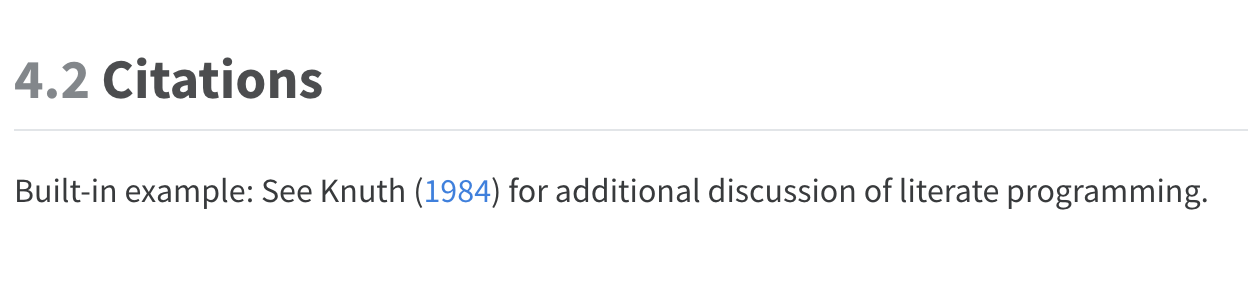
\includegraphics{chapters/cross_references/default_citation.png}

}

\caption{\label{fig-default-citation}An example of Quarto's default
citation style.}

\end{figure}%

Here is what the default \texttt{@knuth84} \emph{reference} looks like
after rendering this document.

\begin{figure}[H]

{\centering 
\includegraphics{chapters/cross_references/default_reference.png}

}

\caption{An example of Quarto's default reference style.}

\end{figure}%

Here is what the \texttt{@knuth84} \emph{citation} above looks like
after changing the citation style to AMA and rendering this document.

\begin{figure}

\centering{


\includegraphics{chapters/cross_references/ama_citation.png}

}

\caption{\label{fig-ama-citation}An example of an AMA citation.}

\end{figure}%

Here is what the \texttt{@knuth84} \emph{reference} looks like after
changing the citation style to AMA and rendering this document.

\begin{figure}

\centering{


\includegraphics{chapters/cross_references/ama_reference.png}

}

\caption{\label{fig-ama-reference}An example of an AMA reference.}

\end{figure}%

🔴 Try integrating Zotero. -
\href{https://github.com/orgs/brad-cannell/projects/3/views/4?pane=issue&itemId=75494998}{GitHub
issue} -
\href{https://quarto.org/docs/visual-editor/options.html\#citation-options}{Quarto
documentation}

\section{Footnotes}\label{footnotes}

I haven't done a lot of footnotes in the past, but
\href{https://quarto.org/docs/authoring/footnotes-and-citations.html\#footnotes}{here
is some documentation} in case I want to do them in the
future.\footnote{And here is an example footnote.}

\section{Glossary}\label{glossary}

Following the emphasizing text guidance in the
\href{https://github.com/brad-cannell/r4epi/wiki/Emphasizing-Text}{R4Epi
Wiki}, we sometimes want to hyperlink words that we will define in the
\href{../appendices/glossary.qmd}{Glossary}. We can definitely link
selected words in the narrative of the chapters to \emph{headings}, but
that approach creates a line in the table of contents for each word in
the glossary, which isn't ideal. I posted this issue on
\href{https://stackoverflow.com/questions/76691907/quarto-link-a-word-in-one-qmd-document-to-a-word-in-a-different-qmd-document/76719362\#76719362}{Stack
Overflow}. Therefore, the best strategy so far seems to be using
\href{https://pandoc.org/MANUAL.html\#definition-lists}{definition
lists}.

For example, let's say that we want to define the term
\href{../appendices/glossary.qmd}{data frame} in the glossary. The first
thing we do is assign and CSS ID to the word ``data frame'' in the
glossary qmd file. For now, I'm planning to prefix all glossary IDs with
the word ``glossary'' in case I need to search for them later.

\begin{Shaded}
\begin{Highlighting}[]
\CommentTok{[}\OtherTok{Data frame}\CommentTok{]}\NormalTok{\{\#glossary{-}data{-}frame\} }

\NormalTok{:  For our purposes, data frames are just R\textquotesingle{}s term for data set or data table. Data frames are made up of columns (variables) and rows (observations). In R, all columns of a data frame must have the same length.}
\end{Highlighting}
\end{Shaded}

\begin{tcolorbox}[enhanced jigsaw, breakable, title=\textcolor{quarto-callout-important-color}{\faExclamation}\hspace{0.5em}{Definition lists}, bottomrule=.15mm, coltitle=black, left=2mm, colbacktitle=quarto-callout-important-color!10!white, colback=white, toprule=.15mm, leftrule=.75mm, arc=.35mm, colframe=quarto-callout-important-color-frame, bottomtitle=1mm, toptitle=1mm, opacityback=0, titlerule=0mm, opacitybacktitle=0.6, rightrule=.15mm]

The colon followed by two spaces before the term's definition is not
optional.

\end{tcolorbox}

Next, use a hyperlink to reference the glossary term in the narrative of
the chapter. For example,

\begin{Shaded}
\begin{Highlighting}[]
\NormalTok{We want to define the term }\CommentTok{[}\OtherTok{data frame}\CommentTok{](../appendices/glossary.qmd\#glossary{-}data{-}frame)}\NormalTok{ in the glossary.}
\end{Highlighting}
\end{Shaded}

Which looks like this: We want to define the term
\hyperref[glossary-data-frame]{data frame} in the glossary.

Additionally, terms linked in this way should also work in PDF
downloads.

If we want to adjust the style of the of the glossary term (e.g.,
increase the font size or make it bold), we can do so in the
\texttt{.scss} file. For example,

\begin{Shaded}
\begin{Highlighting}[]
\NormalTok{dl \{}
  \KeywordTok{font{-}size}\CharTok{:} \DecValTok{14}\DataTypeTok{pt}\OperatorTok{;}
  \KeywordTok{font{-}weight}\CharTok{:} \DecValTok{bold}\OperatorTok{;}
\NormalTok{\}}
\end{Highlighting}
\end{Shaded}

We use \texttt{dl} because Pandoc renders the HTML output to description
list (\texttt{\textless{}dl\textgreater{}}) elements. This styling
should also work in PDF downloads.

\chapter{Custom Styling}\label{sec-custom-styling}

Useful websites:

\begin{itemize}
\tightlist
\item
  \href{https://quarto.org/docs/output-formats/html-themes.html}{Quarto
  documentation on HTML theming}
\item
  \href{https://ucsb-meds.github.io/customizing-quarto-websites/\#/title-slide}{Customizing
  Quarto Websites}
\end{itemize}

In the Bookdown version of R4Epi, I had a custom CSS stylesheet (i.e.,
\texttt{style.css}) that I used create some custom call-out boxes and a
few other things. Here is the contents of that stylesheet.

\begin{Shaded}
\begin{Highlighting}[]
\InformationTok{\textasciigrave{}\textasciigrave{}\textasciigrave{}\{css\}}

\InformationTok{/******************************************************************************}
\InformationTok{CSS for the R4Epi textbook}
\InformationTok{******************************************************************************/}

\InformationTok{/*}
\InformationTok{CSS that came with bookdown}
\InformationTok{*/}
\InformationTok{p.caption \{}
\InformationTok{  color: \#777;}
\InformationTok{  margin{-}top: 10px;}
\InformationTok{\}}
\InformationTok{p code \{}
\InformationTok{  white{-}space: inherit;}
\InformationTok{\}}
\InformationTok{pre \{}
\InformationTok{  word{-}break: normal;}
\InformationTok{  word{-}wrap: normal;}
\InformationTok{\}}
\InformationTok{pre code \{}
\InformationTok{  white{-}space: inherit;}
\InformationTok{\}}

\InformationTok{/* }
\InformationTok{Font Styles}
\InformationTok{*/}
\InformationTok{.large{-}bold \{}
\InformationTok{  font{-}size: 2em;}
\InformationTok{  font{-}weight: bold;}
\InformationTok{\}}

\InformationTok{.underline \{}
\InformationTok{  text{-}decoration: underline;}
\InformationTok{\}}

\InformationTok{.red{-}text \{}
\InformationTok{  color: red;}
\InformationTok{\}}

\InformationTok{.code \{}
\InformationTok{  color: \#0365C0;}
\InformationTok{  font{-}family: "Courier New", Courier, monospace;}
\InformationTok{\}}


\InformationTok{/*}
\InformationTok{Note styles}
\InformationTok{*/}
\InformationTok{.note \{}
\InformationTok{  {-}moz{-}border{-}radius: 6px;}
\InformationTok{  {-}webkit{-}border{-}radius: 6px;}
\InformationTok{  background{-}color: \#f0f7fb;}
\InformationTok{  border: solid 1px \#3498db;}
\InformationTok{  border{-}radius: 6px;}
\InformationTok{  line{-}height: 18px;}
\InformationTok{  overflow: hidden;}
\InformationTok{  padding: 15px 15px;}
\InformationTok{\}}

\InformationTok{.warning \{}
\InformationTok{  {-}moz{-}border{-}radius: 6px;}
\InformationTok{  {-}webkit{-}border{-}radius: 6px;}
\InformationTok{  background{-}color: \#FEFBEA;}
\InformationTok{  border: solid 1px \#F2E394;}
\InformationTok{  border{-}radius: 6px;}
\InformationTok{  line{-}height: 18px;}
\InformationTok{  overflow: hidden;}
\InformationTok{  padding: 15px 15px;}
\InformationTok{\}}


\InformationTok{/* }
\InformationTok{Text box with construction stripes for chapters under construction.}
\InformationTok{Helpful websites: }
\InformationTok{https://css{-}tricks.com/stripes{-}css/}
\InformationTok{https://stackoverflow.com/questions/10422949/css{-}background{-}opacity}
\InformationTok{*/}
\InformationTok{.under{-}construction \{}
\InformationTok{  {-}moz{-}border{-}radius: 6px;}
\InformationTok{  {-}webkit{-}border{-}radius: 6px;}
\InformationTok{  /*background{-}color: rgba(248, 116, 49, 0.4);*/ /* Fourth number is opacity */}
\InformationTok{  background: repeating{-}linear{-}gradient(}
\InformationTok{    45deg,}
\InformationTok{    rgba(248, 116, 49, 0.1) /* Fourth number is opacity */,}
\InformationTok{    rgba(248, 116, 49, 0.1) 10px,}
\InformationTok{    rgba(169, 169, 169, 0.15) 10px,}
\InformationTok{    rgba(169, 169, 169, 0.15) 20px}
\InformationTok{  );}
\InformationTok{  border: solid 1px \#F87431;}
\InformationTok{  border{-}radius: 6px;}
\InformationTok{  line{-}height: 26px;}
\InformationTok{  overflow: hidden;}
\InformationTok{  padding: 15px 15px;}
\InformationTok{  font{-}size: 24px;}
\InformationTok{\}}


\InformationTok{/*}
\InformationTok{Disable the title header from the index page.}
\InformationTok{https://stackoverflow.com/questions/53399095/disable{-}title{-}author{-}in{-}the{-}html{-}output{-}of{-}bookdown}
\InformationTok{*/}
\InformationTok{\#header \{}
\InformationTok{    display: none;}
\InformationTok{\}}

\InformationTok{\textasciigrave{}\textasciigrave{}\textasciigrave{}}
\end{Highlighting}
\end{Shaded}

Following the guidance on
\href{https://ucsb-meds.github.io/customizing-quarto-websites/\#/title-slide}{Customizing
Quarto Websites}, I'm going use that stylesheet for this book too.

\begin{Shaded}
\begin{Highlighting}[]
\InformationTok{\textasciigrave{}\textasciigrave{}\textasciigrave{}\{scss\}}

\InformationTok{/******************************************************************************}
\InformationTok{Custom CSS styling for the Test Quarto Book}
\InformationTok{******************************************************************************/}

\InformationTok{/*{-}{-} scss:defaults {-}{-}*/}

\InformationTok{// Fonts}
\InformationTok{// Importing a font from Google Fonts (https://ucsb{-}meds.github.io/customizing{-}quarto{-}websites/\#/select{-}fonts)}
\InformationTok{// @import url(\textquotesingle{}https://fonts.googleapis.com/css2?family=Roboto:wght@100\&display=swap\textquotesingle{}); // For testing}
\InformationTok{$codeFont:  "Courier New", Courier, monospace;}

\InformationTok{// Colors}
\InformationTok{// $purple: \#AE8BD1; // For testing}
\InformationTok{$codeBackground: \#0365C0;}
\InformationTok{$noteBackground: \#f0f7fb;}
\InformationTok{$noteBorder: \#3498db;}
\InformationTok{$warningBackground: \#FEFBEA;}
\InformationTok{$warningBorder: \#F2E394;}

\InformationTok{// Adjustments to default Quarto styles}
\InformationTok{// $body{-}bg: $purple; // page background {-}{-} for testing}


\InformationTok{/*{-}{-} My Font Styles {-}{-}*/}
\InformationTok{.large{-}bold \{}
\InformationTok{  font{-}size: 2em;}
\InformationTok{  font{-}weight: bold;}
\InformationTok{\}}

\InformationTok{.underline \{}
\InformationTok{  text{-}decoration: underline;}
\InformationTok{\}}

\InformationTok{.red{-}text \{}
\InformationTok{  color: red;}
\InformationTok{\}}

\InformationTok{.code \{}
\InformationTok{  color: $codeBackground;}
\InformationTok{  font{-}family: $codeFont;}
\InformationTok{\}}


\InformationTok{/*{-}{-} Note Styles {-}{-}*/}
\InformationTok{.note \{}
\InformationTok{  {-}moz{-}border{-}radius: 6px;}
\InformationTok{  {-}webkit{-}border{-}radius: 6px;}
\InformationTok{  background{-}color: $noteBackground;}
\InformationTok{  border: solid 1px $noteBorder;}
\InformationTok{  border{-}radius: 6px;}
\InformationTok{  line{-}height: 18px;}
\InformationTok{  overflow: hidden;}
\InformationTok{  padding: 15px 15px;}
\InformationTok{\}}

\InformationTok{.warning \{}
\InformationTok{  {-}moz{-}border{-}radius: 6px;}
\InformationTok{  {-}webkit{-}border{-}radius: 6px;}
\InformationTok{  background{-}color: $warningBackground;}
\InformationTok{  border: solid 1px $warningBorder;}
\InformationTok{  border{-}radius: 6px;}
\InformationTok{  line{-}height: 18px;}
\InformationTok{  overflow: hidden;}
\InformationTok{  padding: 15px 15px;}
\InformationTok{\}}


\InformationTok{/* }
\InformationTok{Text box with construction stripes for chapters under construction.}
\InformationTok{Helpful websites: }
\InformationTok{https://css{-}tricks.com/stripes{-}css/}
\InformationTok{https://stackoverflow.com/questions/10422949/css{-}background{-}opacity}

\InformationTok{I could create SASS variables for these elements, but I don\textquotesingle{}t want to take the time to do that now.}
\InformationTok{*/}
\InformationTok{.under{-}construction \{}
\InformationTok{  {-}moz{-}border{-}radius: 6px;}
\InformationTok{  {-}webkit{-}border{-}radius: 6px;}
\InformationTok{  /*background{-}color: rgba(248, 116, 49, 0.4);*/ /* Fourth number is opacity */}
\InformationTok{  background: repeating{-}linear{-}gradient(}
\InformationTok{    45deg,}
\InformationTok{    rgba(248, 116, 49, 0.1) /* Fourth number is opacity */,}
\InformationTok{    rgba(248, 116, 49, 0.1) 10px,}
\InformationTok{    rgba(169, 169, 169, 0.15) 10px,}
\InformationTok{    rgba(169, 169, 169, 0.15) 20px}
\InformationTok{  );}
\InformationTok{  border: solid 1px \#F87431;}
\InformationTok{  border{-}radius: 6px;}
\InformationTok{  line{-}height: 26px;}
\InformationTok{  overflow: hidden;}
\InformationTok{  padding: 15px 15px;}
\InformationTok{  font{-}size: 24px;}
\InformationTok{\}}


\InformationTok{/*}
\InformationTok{Disable the title header from the index page.}
\InformationTok{https://stackoverflow.com/questions/53399095/disable{-}title{-}author{-}in{-}the{-}html{-}output{-}of{-}bookdown}
\InformationTok{*/}
\InformationTok{\#header \{}
\InformationTok{    display: none;}
\InformationTok{\}}

\InformationTok{\textasciigrave{}\textasciigrave{}\textasciigrave{}}
\end{Highlighting}
\end{Shaded}

For testing, I'm going to add a note, a warning, and a construction box.

🗒\textbf{Side Note:} Here is a note.

\begin{Shaded}
\begin{Highlighting}[]
\DataTypeTok{\textless{}}\KeywordTok{p}\OtherTok{ class}\OperatorTok{=}\StringTok{"note"}\DataTypeTok{\textgreater{}}\NormalTok{ 🗒**Side Note:** Here is a note. }\DataTypeTok{\textless{}/}\KeywordTok{p}\DataTypeTok{\textgreater{}}
\end{Highlighting}
\end{Shaded}

⚠️\textbf{Warning:} Here is a warning.

\begin{Shaded}
\begin{Highlighting}[]
\DataTypeTok{\textless{}}\KeywordTok{p}\OtherTok{ class}\OperatorTok{=}\StringTok{"warning"}\DataTypeTok{\textgreater{}}\NormalTok{ ⚠️**Warning:** Here is a warning. }\DataTypeTok{\textless{}/}\KeywordTok{p}\DataTypeTok{\textgreater{}}
\end{Highlighting}
\end{Shaded}

\texttt{r\ fontawesome::fa("hammer",\ fill\ =\ "\#000000",\ height="1em")}
Here is the under construction box.

\begin{Shaded}
\begin{Highlighting}[]
\DataTypeTok{\textless{}}\KeywordTok{p}\OtherTok{ class}\OperatorTok{=}\StringTok{"under{-}construction"}\DataTypeTok{\textgreater{}}\NormalTok{ \textasciigrave{}r fontawesome::fa("hammer", fill = "\#000000", height="1em")\textasciigrave{} Here is the under construction box.}\DataTypeTok{\textless{}/}\KeywordTok{p}\DataTypeTok{\textgreater{}}
\end{Highlighting}
\end{Shaded}

Note that Font Awesome is not currently working and none of these call
out boxes work in PDF format. Quarto's built-in call out boxes do work
in PDF format, though.

\section{Font Awesome}\label{font-awesome}

\href{https://fontawesome.com/}{Font Awesome} seems like a great tool
for adding an additional visual dimension to our Quarto projects. Here
are some links with useful information about adding Font Awesome
graphics to Quarto documents:

\begin{itemize}
\tightlist
\item
  How to include fontawesome icons in Quarto documents: basic styling
  AND special effects
  (\href{https://www.youtube.com/watch?v=u8EOVOjX13Y}{YouTube})
\end{itemize}

Here are the basics:

\begin{enumerate}
\def\labelenumi{\arabic{enumi}.}
\tightlist
\item
  Install the Font Awesome Quarto Extension by typing
  \texttt{quarto\ install\ extension\ quarto-ext/fontawesome} in the
  terminal.
\item
  We will be asked, ``Do you trust the authors of this extension?'' Type
  ``Yes.''
\item
  We will be asked, ``Would you like to continue?'' Type ``Yes.''
\item
  There should be a new folder called \texttt{\_extensions}. Inside that
  folder, there should be a folder named \texttt{fontawesome}.
\item
  We will have to repeat this process any time we create a new Quarto
  project.
\end{enumerate}

Now that the extension is installed, we can use the following syntax to
insert Font Awesome icons:
\texttt{\textbackslash{}\{\textbackslash{}\{\textless{}\ fa\ name-of-icon\ \textgreater{}\}\}}
(don't include the backslashes. They are just there to prevent GitHub
from attempting to render the code). We can find a list of icons on the
\href{https://fontawesome.com/search}{Font Awesome website}.

For example, this code creates a Font Awesome envelope:
\faIcon{envelope}

\begin{Shaded}
\begin{Highlighting}[]
\SpecialCharTok{\textbackslash{}\{\textbackslash{}\{}\NormalTok{\textless{} fa envelope \textgreater{}\}\} (don\textquotesingle{}t include the backslashes. They are just there to prevent GitHub from attempting to render the code)}
\end{Highlighting}
\end{Shaded}

However, the example above doesn't work when we render the file to
GitHub flavored markdown (\texttt{format:\ gfm}) instead of html
(\texttt{format:\ html}).

Here are some links with notes on using Font Awesome with GitHub
flavored markdown:

\begin{itemize}
\tightlist
\item
  Add to markdown:
  https://stackoverflow.com/questions/63913973/how-can-i-put-fontawesome-icons-in-markdown-readme
\item
  GitHub repository: https://github.com/FortAwesome/Font-Awesome
\item
  R font awesome package: https://github.com/rstudio/fontawesome
\end{itemize}

For example:

\begin{Shaded}
\begin{Highlighting}[]
\NormalTok{\textless{}img src="https://raw.githubusercontent.com/FortAwesome/Font{-}Awesome/6.x/svgs/solid/crown.svg" width="50" height="50"\textgreater{}}
\end{Highlighting}
\end{Shaded}

Produces:

The YouTube video,
\href{https://www.youtube.com/watch?v=u8EOVOjX13Y}{How to include
fontawesome icons in Quarto documents: basic styling AND special
effects} has more information on styling Font Awesome icons. For
example, the following code:

\begin{Shaded}
\begin{Highlighting}[]
\NormalTok{\textless{}div class="fa{-}3x"\textgreater{}}
\NormalTok{  \textless{}i class="fa{-}solid fa{-}circle{-}plus fa{-}beat"\textgreater{}\textless{}/i\textgreater{}}
\NormalTok{  \textless{}i class="fa{-}solid fa{-}heart fa{-}beat"\textgreater{}\textless{}/i\textgreater{}}
\NormalTok{  \textless{}i class="fa{-}solid fa{-}heart fa{-}beat" style="{-}{-}fa{-}animation{-}duration: 0.5s;" \textgreater{}\textless{}/i\textgreater{}}
\NormalTok{  \textless{}i class="fa{-}solid fa{-}heart fa{-}beat" style="{-}{-}fa{-}animation{-}duration: 2s;"\textgreater{}\textless{}/i\textgreater{}}
\NormalTok{  \textless{}i class="fa{-}solid fa{-}heart fa{-}beat" style="{-}{-}fa{-}beat{-}scale: 2.0;"\textgreater{}\textless{}/i\textgreater{}}
\NormalTok{\textless{}/div\textgreater{}}
\end{Highlighting}
\end{Shaded}

Produces this:

\textbf{Note on rendering to PDF:} The double curly brace syntax renders
in the PDF document, but the HTML code does not.

\textbf{Another weird thing:} When I was trying to include fontawesome
icons in the ``About the Authors'' page of the Quarto version of R4Epi,
I found that I had to include at least one code chunk in the file to get
the fontawesome icons to render. Here is an example of the code I used
that included fontawesome icons:

\begin{Shaded}
\begin{Highlighting}[]
\NormalTok{\textless{}a href="https://www.bradcannell.com" target="\_blank"\textgreater{}}\InformationTok{\textasciigrave{}r fontawesome::fa("globe", fill = "\#003087", height="2em")\textasciigrave{}}\NormalTok{\textless{}/a\textgreater{}}
\end{Highlighting}
\end{Shaded}

\chapter{Gifs}\label{sec-gifs}

In R4Epi, we use quite a few gifs. That makes rendering the book to pdf
format challenging. What happens when we add a gif to a qmd document and
render it to pdf?

The following code works great for HTML format, but it messes up pdf
format.

\begin{Shaded}
\begin{Highlighting}[]
\AlertTok{![A gif about file paths](img/file\_path\_gif.gif)}\NormalTok{\{\#fig{-}file{-}paths\}}

\NormalTok{And I can }\CommentTok{[}\OtherTok{cross reference}\CommentTok{](https://quarto.org/docs/authoring/cross{-}references.html)}\NormalTok{ the gif by typing }\InformationTok{\textasciigrave{}@fig{-}file{-}paths\textasciigrave{}}\NormalTok{. See @fig{-}file{-}paths}

\NormalTok{::: \{.callout{-}important\}}
\NormalTok{For cross{-}references to work, the image must have a caption \_and\_ a label.}
\NormalTok{:::}
\end{Highlighting}
\end{Shaded}

What if I use \texttt{knitr::include\_graphics("path")}?

\begin{Shaded}
\begin{Highlighting}[]

\InformationTok{\textasciigrave{}\textasciigrave{}\textasciigrave{}\{r\}}
\InformationTok{\#| label: fig{-}file{-}paths}
\InformationTok{\#| echo: false}
\InformationTok{\#| fig{-}cap: |}
\InformationTok{\#|   A gif about file paths.}
\InformationTok{\#| fig{-}alt: |}
\InformationTok{\#|   A gif about file paths.}

\InformationTok{knitr::include\_graphics("file\_path\_gif.gif")}
\InformationTok{\textasciigrave{}\textasciigrave{}\textasciigrave{}}

\NormalTok{And I can }\CommentTok{[}\OtherTok{cross reference}\CommentTok{](https://quarto.org/docs/authoring/cross{-}references.html)}\NormalTok{ the figure by typing }\InformationTok{\textasciigrave{}@fig{-}file{-}paths\textasciigrave{}}\NormalTok{. See @fig{-}file{-}paths}

\NormalTok{::: \{.callout{-}important\}}
\NormalTok{For cross{-}references to work, the image must have a caption \_and\_ a label.}
\NormalTok{:::}
\end{Highlighting}
\end{Shaded}

No, this doesn't work either.
\href{https://github.com/quarto-dev/quarto-cli/discussions/3551}{Here is
a pretty good discussion on the topic}. It looks like the easiest route
may be to use
\href{https://quarto.org/docs/authoring/conditional.html}{conditional
content}. Given the limited number of gifs in R4Epi, this shouldn't be
too big of a problem.

So, start by conditionally displaying the gif if the output format is
html.

\begin{Shaded}
\begin{Highlighting}[]

\NormalTok{::: \{.content{-}visible when{-}format="html"\}}

\InformationTok{\textasciigrave{}\textasciigrave{}\textasciigrave{}\{r\}}
\InformationTok{\#| label: fig{-}file{-}paths}
\InformationTok{\#| echo: false}
\InformationTok{\#| fig{-}cap: |}
\InformationTok{\#|   A gif about file paths.}
\InformationTok{\#| fig{-}alt: |}
\InformationTok{\#|   A gif about file paths.}

\InformationTok{knitr::include\_graphics("file\_path\_gif.gif")}
\InformationTok{\textasciigrave{}\textasciigrave{}\textasciigrave{}}

\NormalTok{:::}
\end{Highlighting}
\end{Shaded}

Which renders as\ldots{}

Then, conditionally add a thumbnail image of the gif when the output
format is pdf.

\begin{itemize}
\tightlist
\item
  Create a duplicate of the gif in Finder.
\item
  Add ``\_thumb'' to the end of the file name (before the file
  extension).
\item
  Open the duplicate file in preview.
\item
  Use Preview's sidebar to keep only one of the thumbnail images from
  the gif (select and delete the rest).
\item
  Click File \textgreater{} Export and export to png.
\item
  Delete the duplicate gif.
\end{itemize}

\begin{Shaded}
\begin{Highlighting}[]

\NormalTok{::: \{.content{-}visible when{-}format="pdf"\}}

\InformationTok{\textasciigrave{}\textasciigrave{}\textasciigrave{}\{r\}}
\InformationTok{\#| label: fig{-}file{-}paths}
\InformationTok{\#| echo: false}
\InformationTok{\#| fig{-}cap: |}
\InformationTok{\#|   A thumbnail of gif about file paths.}
\InformationTok{\#| fig{-}alt: |}
\InformationTok{\#|   A thumbnail gif about file paths.}

\InformationTok{knitr::include\_graphics("file\_path\_gif.gif")}
\InformationTok{\textasciigrave{}\textasciigrave{}\textasciigrave{}}

\NormalTok{:::}
\end{Highlighting}
\end{Shaded}

Which renders as\ldots{}

\begin{figure}

\centering{

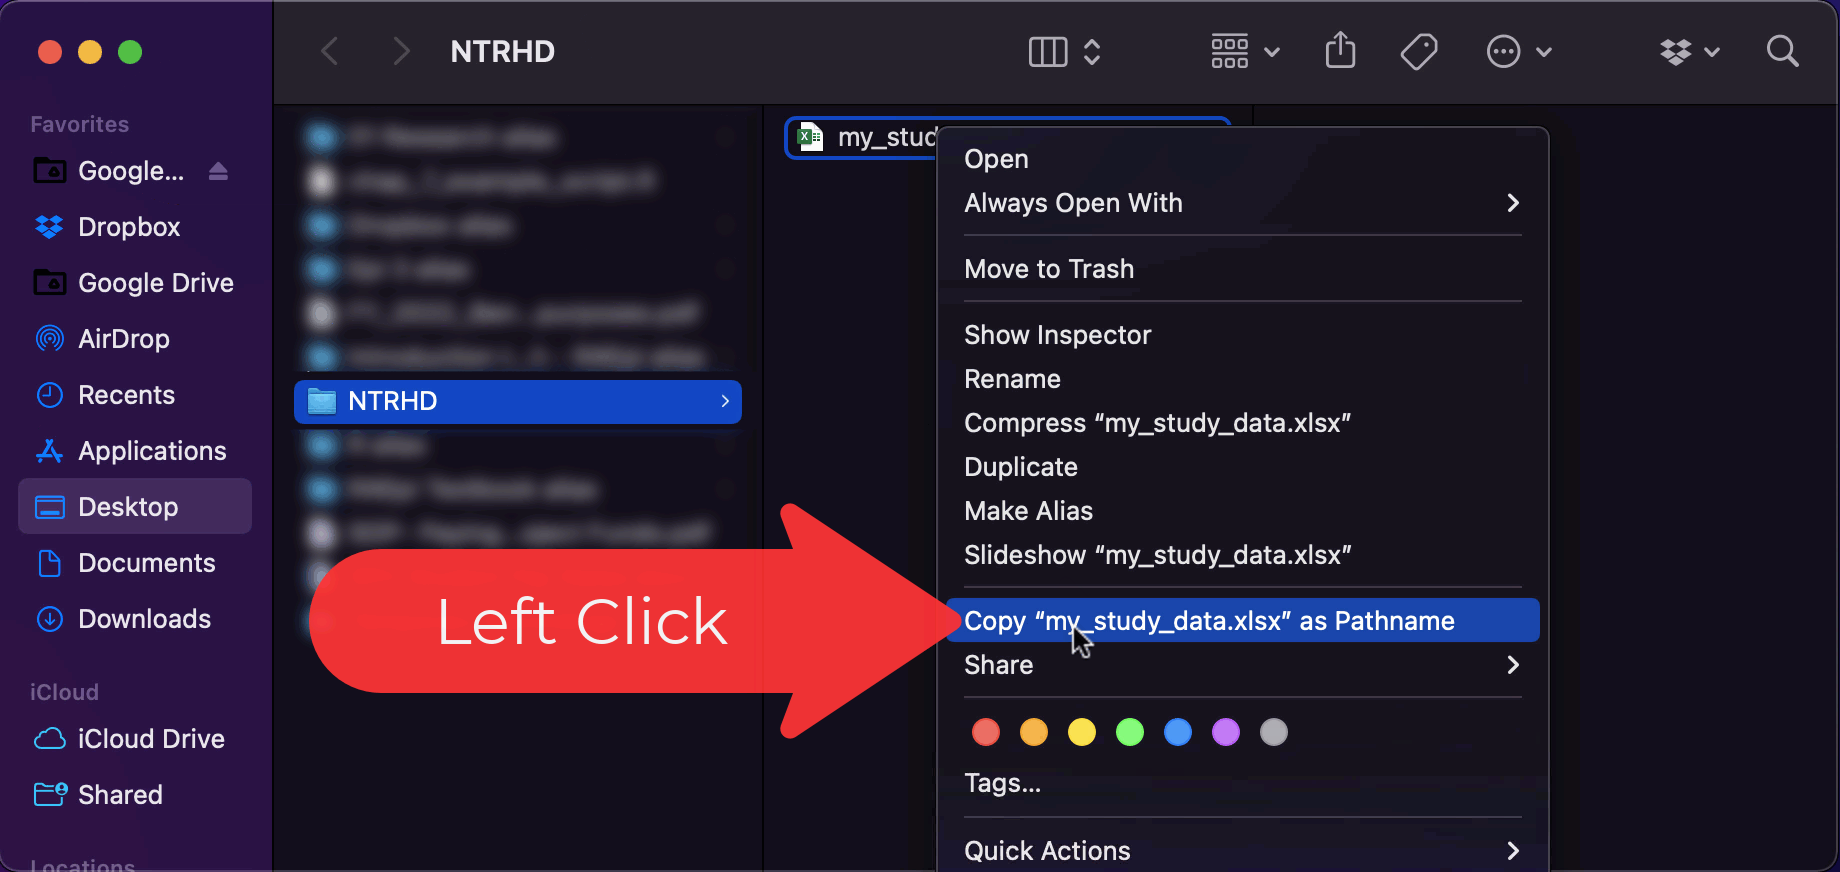
\includegraphics[width=6.13in,height=\textheight]{chapters/gifs/file_path_gif_thumb.png}

}

\caption{\label{fig-file-paths_thumb}A thumbnail of gif about file
paths.}

\end{figure}%

\chapter{Google Sheets}\label{google-sheets}

These are notes on authoring Quarto documents with Google Sheets.

\section{Embedding Google Sheets}\label{embedding-google-sheets}

I'm following instructions from
\href{https://support.google.com/docs/thread/212358523/embedding-a-table-from-sheets-to-a-website?hl=en}{this
post}.

\begin{enumerate}
\def\labelenumi{\arabic{enumi}.}
\item
  We created an
  \href{https://docs.google.com/spreadsheets/d/1RVgT28QJ6dV5kCSzS9BEOVMooiy06DEhv2d-eqxIjZY/edit?gid=0\#gid=0}{example
  Google Sheet} to embed.
\item
  Click \texttt{Help} \textgreater{} \texttt{Search\ the\ menus}
  \textgreater{} \texttt{Publish\ to\ the\ web}.
\item
  Click \texttt{Embed} and choose \texttt{Entire\ Document} or a
  specific sheet. We will test both bellow.
\item
  Click \texttt{Publish} and copy the embed code.
\end{enumerate}

\subsection{Embed the entire document}\label{embed-the-entire-document}

\begin{tcolorbox}[enhanced jigsaw, breakable, title=\textcolor{quarto-callout-note-color}{\faInfo}\hspace{0.5em}{Note}, bottomrule=.15mm, coltitle=black, left=2mm, colbacktitle=quarto-callout-note-color!10!white, colback=white, toprule=.15mm, leftrule=.75mm, arc=.35mm, colframe=quarto-callout-note-color-frame, bottomtitle=1mm, toptitle=1mm, opacityback=0, titlerule=0mm, opacitybacktitle=0.6, rightrule=.15mm]

The Google sheet will not appear in the PDF version of this SOP.

\end{tcolorbox}

\subsection{Embed a single sheet}\label{embed-a-single-sheet}

\begin{tcolorbox}[enhanced jigsaw, breakable, title=\textcolor{quarto-callout-note-color}{\faInfo}\hspace{0.5em}{Note}, bottomrule=.15mm, coltitle=black, left=2mm, colbacktitle=quarto-callout-note-color!10!white, colback=white, toprule=.15mm, leftrule=.75mm, arc=.35mm, colframe=quarto-callout-note-color-frame, bottomtitle=1mm, toptitle=1mm, opacityback=0, titlerule=0mm, opacitybacktitle=0.6, rightrule=.15mm]

The Google sheet will not appear in the PDF version of this SOP.

\end{tcolorbox}

\chapter{Images}\label{sec-images}

Here are some examples of adding figures.

Links

\begin{itemize}
\tightlist
\item
  \href{https://quarto.org/docs/authoring/figures.html}{The Quarto
  documentation about images}
\item
  \href{https://github.com/hadley/r4ds/blob/main/intro.qmd}{Example
  image in R4DS}
\end{itemize}

\section{Native Quarto figures}\label{native-quarto-figures}

We can use the
\texttt{!{[}Caption\ text{]}(file\_path.png)\{\#fig-label\}} syntax to
add images. For example:

\begin{Shaded}
\begin{Highlighting}[]
\AlertTok{![Relative Path Directions](directions\_relative.png)}\NormalTok{\{\#fig{-}directions\}}
\end{Highlighting}
\end{Shaded}

Renders as:

\begin{figure}

\centering{

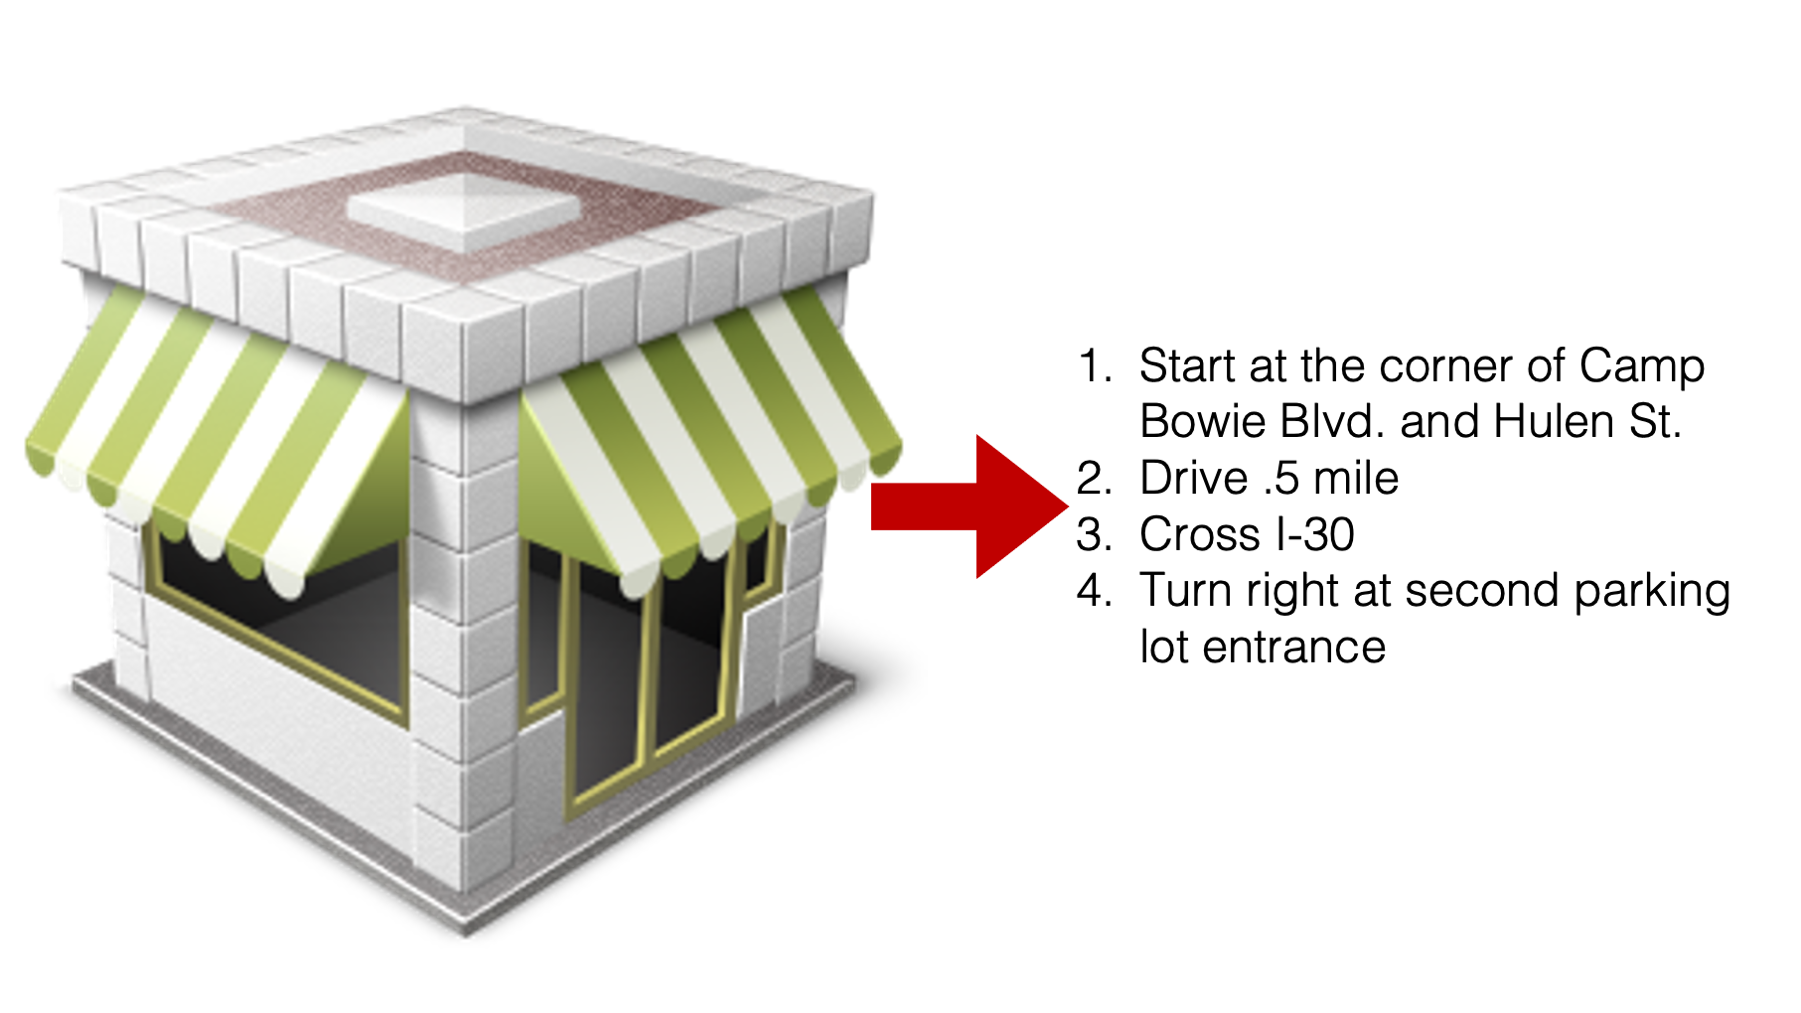
\includegraphics{chapters/images/directions_relative.png}

}

\caption{\label{fig-directions}Relative Path Directions}

\end{figure}%

And I can
\href{https://quarto.org/docs/authoring/cross-references.html}{cross
reference} the figure by typing \texttt{@fig-directions}. See
Figure~\ref{fig-directions}

\begin{tcolorbox}[enhanced jigsaw, breakable, title=\textcolor{quarto-callout-important-color}{\faExclamation}\hspace{0.5em}{Important}, bottomrule=.15mm, coltitle=black, left=2mm, colbacktitle=quarto-callout-important-color!10!white, colback=white, toprule=.15mm, leftrule=.75mm, arc=.35mm, colframe=quarto-callout-important-color-frame, bottomtitle=1mm, toptitle=1mm, opacityback=0, titlerule=0mm, opacitybacktitle=0.6, rightrule=.15mm]

For cross-references to work, the image must have a caption \emph{and} a
label.

\end{tcolorbox}

\section{Adding figures with Knitr}\label{adding-figures-with-knitr}

In R4DS (link above), Hadley et al.~are still using
\texttt{knitr::include\_graphics("path")} to insert images even though
the book has been converted to Quarto documents. When using Bookdown,
\href{https://bookdown.org/yihui/bookdown/figures.html}{Yihui gives four
arguments} for using \texttt{knitr::include\_graphics("path")} instead
of native markdown image formatting. So, we will likely continue to use
them too. Here is an example image code chunk from
\href{https://github.com/hadley/r4ds/blob/main/intro.qmd}{R4DS}:

\begin{Shaded}
\begin{Highlighting}[]
\InformationTok{\textasciigrave{}\textasciigrave{}\textasciigrave{}\{r\}}
\InformationTok{\#| label: fig{-}ds{-}diagram}
\InformationTok{\#| echo: false}
\InformationTok{\#| fig{-}cap: |}
\InformationTok{\#|   In our model of the data science process, you start with data import}
\InformationTok{\#|   and tidying. Next, you understand your data with an iterative cycle of}
\InformationTok{\#|   transforming, visualizing, and modeling. You finish the process }
\InformationTok{\#|   by communicating your results to other humans.}
\InformationTok{\#| fig{-}alt: |}
\InformationTok{\#|   A diagram displaying the data science cycle: Import {-}\textgreater{} Tidy {-}\textgreater{} Understand }
\InformationTok{\#|   (which has the phases Transform {-}\textgreater{} Visualize {-}\textgreater{} Model in a cycle) {-}\textgreater{} }
\InformationTok{\#|   Communicate. Surrounding all of these is Communicate.}
\InformationTok{\#| out.width: NULL}

\InformationTok{knitr::include\_graphics("diagrams/data{-}science/base.png", dpi = 270)}
\InformationTok{\textasciigrave{}\textasciigrave{}\textasciigrave{}}
\end{Highlighting}
\end{Shaded}

Here, I'm adding my own image with
\texttt{knitr::include\_graphics("path")}.

\begin{figure}

\centering{

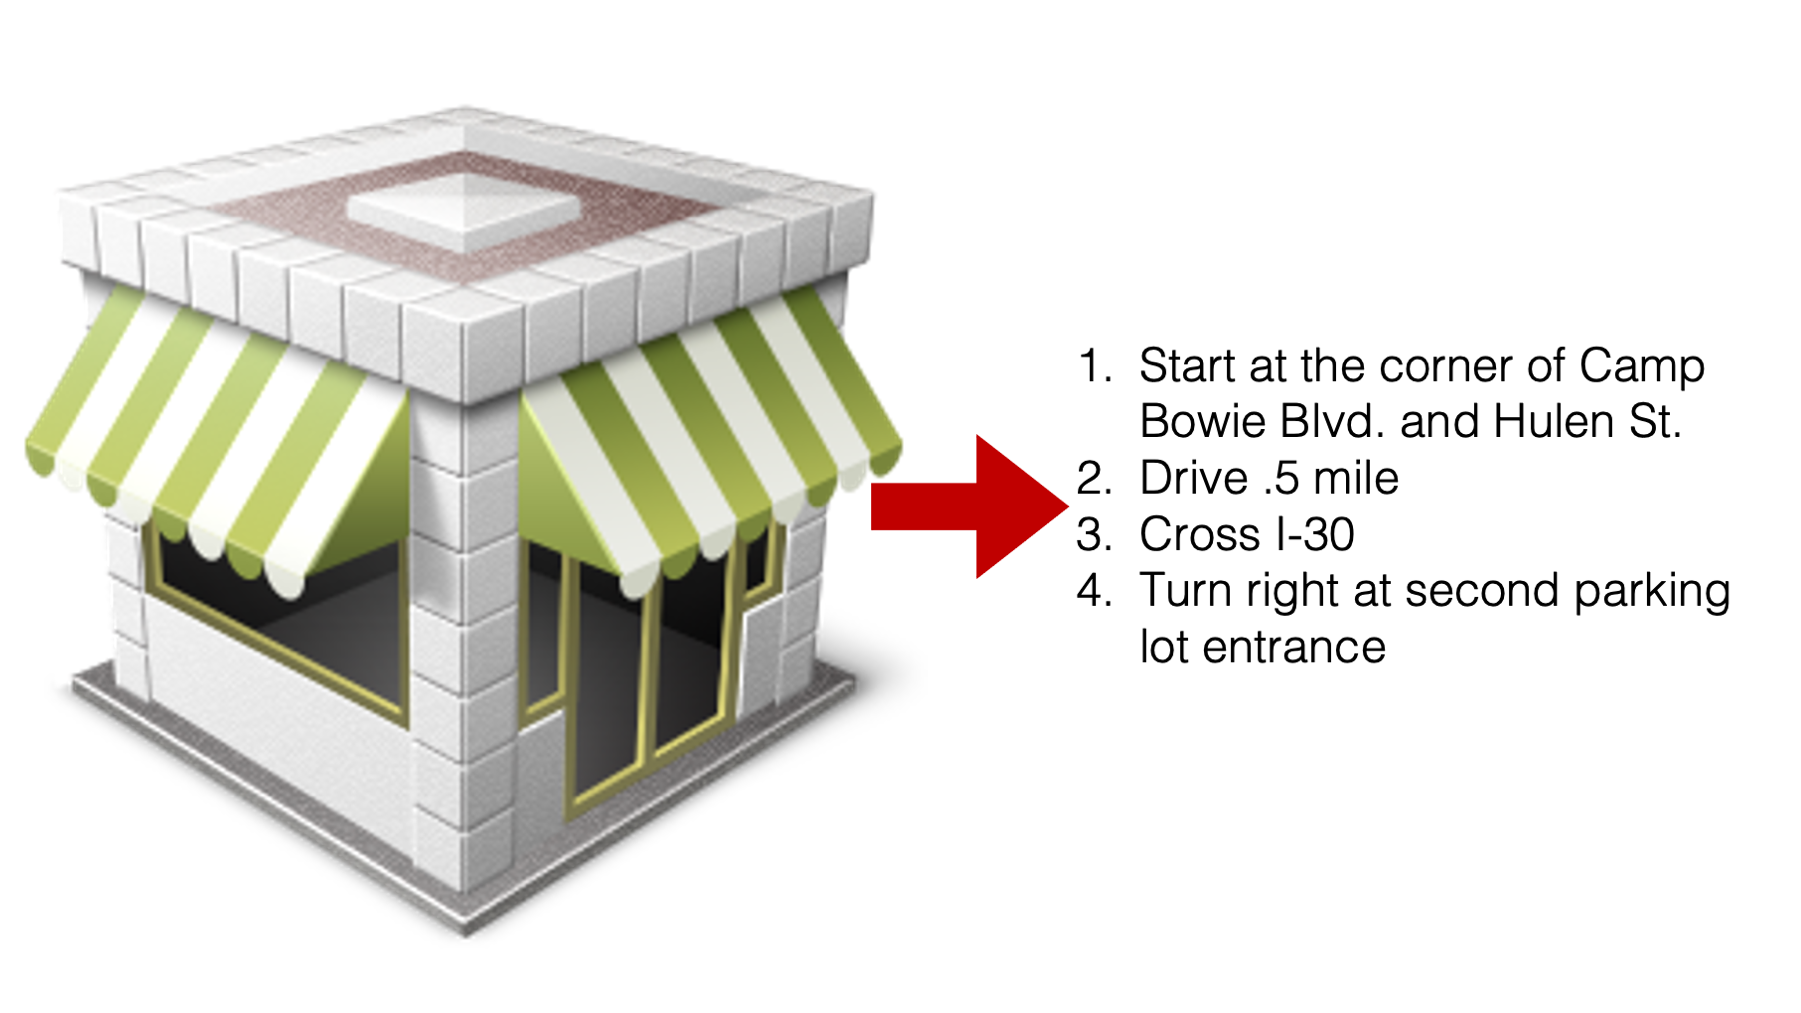
\includegraphics[width=6in,height=\textheight]{chapters/images/directions_relative.png}

}

\caption{\label{fig-directions}Relative Path Directions.}

\end{figure}%

And I can
\href{https://quarto.org/docs/authoring/cross-references.html}{cross
reference} the figure by typing \texttt{@fig-directions}. See
Figure~\ref{fig-directions}

\begin{tcolorbox}[enhanced jigsaw, breakable, title=\textcolor{quarto-callout-important-color}{\faExclamation}\hspace{0.5em}{Important}, bottomrule=.15mm, coltitle=black, left=2mm, colbacktitle=quarto-callout-important-color!10!white, colback=white, toprule=.15mm, leftrule=.75mm, arc=.35mm, colframe=quarto-callout-important-color-frame, bottomtitle=1mm, toptitle=1mm, opacityback=0, titlerule=0mm, opacitybacktitle=0.6, rightrule=.15mm]

For cross-references to work, the image must have a caption \emph{and} a
label.

\end{tcolorbox}

\begin{tcolorbox}[enhanced jigsaw, breakable, title=\textcolor{quarto-callout-warning-color}{\faExclamationTriangle}\hspace{0.5em}{Creating figures without captions}, bottomrule=.15mm, coltitle=black, left=2mm, colbacktitle=quarto-callout-warning-color!10!white, colback=white, toprule=.15mm, leftrule=.75mm, arc=.35mm, colframe=quarto-callout-warning-color-frame, bottomtitle=1mm, toptitle=1mm, opacityback=0, titlerule=0mm, opacitybacktitle=0.6, rightrule=.15mm]

Figure captions will look like \texttt{Figure\ X:\ ?(caption)} if the
chunk label is prefixed with \texttt{fig} (e.g.,
\texttt{\#\textbar{}\ label:\ fig-directions}), but there isn't a valid
\texttt{\#\textbar{}\ fig-cap:}. There are more details given
\href{https://github.com/quarto-dev/quarto-cli/issues/3878}{here}. There
are two ways to resolve this issue:

\begin{enumerate}
\def\labelenumi{\arabic{enumi}.}
\tightlist
\item
  Remove the \texttt{fig-} part of the label.
\item
  Add a valid figure caption.
\end{enumerate}

\end{tcolorbox}

\section{Images}\label{images}

Sometimes I want to add image borders to make the image stand out a
little bit from the background around them. For example, it's kind of
hard to distinguish Figure~\ref{fig-default-citation} from the
text/background around it.

After a quick Google search, there appears to be a
\href{https://quarto.org/docs/authoring/figures.html\#environments}{LaTeX
package} that will add a boarder, but I'm assuming that will only work
for PDF renderings.

Additionally, I imagine that I can probably make some adjustments to the
.scss file that will add boarders to images. However, that should only
work for HTML renderings.

Therefore, the most straightforward and robust option might just be to
add the boarder directly to the image using PowerPoint, Preview,
Photoshop, etc. That's what I did for Figure~\ref{fig-ama-citation}.

\chapter{Rmd Documents}\label{rmd-documents}

I copied this Rmd document over from the Bookdown version of R4Epi
(05\_lets\_get\_programming.Rmd). Just trying to figure out what happens
when we mix and mingle Rmd and qmd documents.

It seems to work well!

\section{Let's Get Programming}\label{lets-get-programming}

In this chapter, we are going to tie together many of the concepts we've
learned so far, and you are going to create your first basic R program.
Specifically, you are going to write a program that simulates some data
and analyzes it.

\section{Simulating data}\label{simulating-data}

Data simulation can be really complicated, but it doesn't have to be. It
is simply the process of \emph{creating} data as opposed to
\emph{finding data in the wild}. This can be really useful in several
different ways.

\begin{enumerate}
\def\labelenumi{\arabic{enumi}.}
\item
  Simulating data is really useful for getting help with a problem you
  are trying to solve. Often, it isn't feasible for you to send other
  people the actual data set you are working on when you encounter a
  problem you need help with. Sometimes, it may not even be legally
  allowed (i.e., for privacy reasons). Instead of sending them your
  entire data set, you can simulate a little data set that recreates the
  challenge you are trying to address without all the other complexity
  of the full data set. As a bonus, I have often found that I end up
  figuring out the solution to the problem I'm trying to solve as I
  recreate the problem in a simulated data set that I intended to share
  with others.
\item
  Simulated data can also be useful for learning about and testing
  statistical assumptions. In epidemiology, we use statistics to draw
  conclusions about populations of people we are interested in based on
  samples of people drawn from the population. Because we don't actually
  have data from \emph{all} the people in the population, we have to
  make some assumptions about the population based on what we find in
  our sample. When we simulate data, we know the truth about our
  population because we \emph{created} our population to have that
  truth. We can then use this simulated population to play ``what if''
  games with our analysis. \emph{What if we only sampled half as many
  people?} \emph{What if their heights aren't actually normally
  distributed?} \emph{What if we used a probit model instead of a logit
  model?} Going through this process and answering these questions can
  help us understand how much, and under what circumstances, we can
  trust the answers we found in the real world.
\end{enumerate}

So, let's go ahead and write a complete R program to simulate and
analyze some data. As I said, it doesn't have to be complicated. In
fact, in just a few lines of R code below we simulate and analyze some
data about a hypothetical class.

\begin{Shaded}
\begin{Highlighting}[]
\NormalTok{class }\OtherTok{\textless{}{-}} \FunctionTok{data.frame}\NormalTok{(}
  \AttributeTok{names   =} \FunctionTok{c}\NormalTok{(}\StringTok{"John"}\NormalTok{, }\StringTok{"Sally"}\NormalTok{, }\StringTok{"Brad"}\NormalTok{, }\StringTok{"Anne"}\NormalTok{),}
  \AttributeTok{heights =} \FunctionTok{c}\NormalTok{(}\DecValTok{68}\NormalTok{, }\DecValTok{63}\NormalTok{, }\DecValTok{71}\NormalTok{, }\DecValTok{72}\NormalTok{)}
\NormalTok{)}
\end{Highlighting}
\end{Shaded}

\begin{Shaded}
\begin{Highlighting}[]
\NormalTok{class}
\end{Highlighting}
\end{Shaded}

\begin{verbatim}
  names heights
1  John      68
2 Sally      63
3  Brad      71
4  Anne      72
\end{verbatim}

\begin{Shaded}
\begin{Highlighting}[]
\FunctionTok{mean}\NormalTok{(class}\SpecialCharTok{$}\NormalTok{heights)}
\end{Highlighting}
\end{Shaded}

\begin{verbatim}
[1] 68.5
\end{verbatim}

As you can see, this data frame contains the students' names and
heights. We also use the \texttt{mean()} function to calculate the
average height of the class. By the end of this chapter, you will
understand all the elements of this R code and how to simulate your own
data.

\section{Vectors}\label{vectors}

Vectors are the most fundamental data structure in R. Here, data
structure means ``container for our data.'' There are other data
structures as well; however, they are all built from vectors. That's why
I say vectors are the most fundamental data structure. Some of these
other structures include matrices, lists, and data frames. In this book,
we won't use matrices or lists much at all, so you can forget about them
for now. Instead, we will almost exclusively use data frames to hold and
manipulate our data. However, because data frames are built from
vectors, it can be useful to start by learning a little bit about them.
Let's create our first vector now.

\begin{Shaded}
\begin{Highlighting}[]
\CommentTok{\# Create an example vector}
\NormalTok{names }\OtherTok{\textless{}{-}} \FunctionTok{c}\NormalTok{(}\StringTok{"John"}\NormalTok{, }\StringTok{"Sally"}\NormalTok{, }\StringTok{"Brad"}\NormalTok{, }\StringTok{"Anne"}\NormalTok{)}
\CommentTok{\# Print contents to the screen}
\NormalTok{names}
\end{Highlighting}
\end{Shaded}

\begin{verbatim}
[1] "John"  "Sally" "Brad"  "Anne" 
\end{verbatim}

👆\textbf{Here's what we did above:}

\begin{itemize}
\item
  We \emph{created} a vector of names with the \texttt{c()} (short for
  combine) function.

  \begin{itemize}
  \item
    The vector contains four values: ``John'', ``Sally'', ``Brad'', and
    ``Anne''.
  \item
    All of the values are character strings (i.e., words). We know this
    because all of the values are wrapped with quotation marks.
  \item
    Here we used double quotes above, but we could have also used single
    quotes. We cannot, however, mix double and single quotes for each
    character string. For example,
    \texttt{c("John\textquotesingle{},\ ...)} won't work.
  \end{itemize}
\item
  We \emph{assigned} that vector of character strings to the word
  \texttt{names} using the \texttt{\textless{}-} function.

  \begin{itemize}
  \item
    R now recognizes \texttt{names} as an \textbf{object} that we can do
    things with.
  \item
    R programmers may refer to the names object as ``the names object'',
    ``the names vector'', or ``the names variable''. For our purposes,
    these all mean the same thing.
  \end{itemize}
\item
  We \emph{printed} the contents of the \texttt{names} object to the
  screen by typing the word ``names''.

  \begin{itemize}
  \tightlist
  \item
    R \textbf{returns} (shows us) the four character values (``John''
    ``Sally'' ``Brad'' ``Anne'') on the computer screen.
  \end{itemize}
\end{itemize}

Try copying and pasting the code above into the RStudio console on your
computer. You should notice the names vector appear in your
\textbf{global environment}. You may also notice that the global
environment pane gives you some additional information about this vector
to the right of its name. Specifically, you should see
\texttt{chr\ {[}1:4{]}\ "John"\ \ "Sally"\ "Brad"\ \ "Anne"}. This is R
telling us that \texttt{names} is a character vector (\texttt{chr}),
with four values (\texttt{{[}1:4{]}}), and the first four values are
\texttt{"John"\ \ "Sally"\ "Brad"\ \ "Anne"}.

\subsection{Vector types}\label{vector-types}

There are several different vector \textbf{types}, but each vector can
have only one type. The type of the vector above was character. We can
validate that with the \texttt{typeof()} function like so:

\begin{Shaded}
\begin{Highlighting}[]
\FunctionTok{typeof}\NormalTok{(names)}
\end{Highlighting}
\end{Shaded}

\begin{verbatim}
[1] "character"
\end{verbatim}

The other vector types that we will use in this book are double,
integer, and logical. Double vectors hold
\href{https://en.wikipedia.org/wiki/Real_number}{real numbers} and
integer vectors hold
\href{https://en.wikipedia.org/wiki/Integer}{integers}. Collectively,
double vectors and integer vectors are known as numeric vectors. Logical
vectors can only hold the values TRUE and FALSE. Here are some examples
of each:

\subsection{Double vectors}\label{double-vectors}

\begin{Shaded}
\begin{Highlighting}[]
\CommentTok{\# A numeric vector}
\NormalTok{my\_numbers }\OtherTok{\textless{}{-}} \FunctionTok{c}\NormalTok{(}\FloatTok{12.5}\NormalTok{, }\FloatTok{13.98765}\NormalTok{, pi)}
\NormalTok{my\_numbers}
\end{Highlighting}
\end{Shaded}

\begin{verbatim}
[1] 12.500000 13.987650  3.141593
\end{verbatim}

\begin{Shaded}
\begin{Highlighting}[]
\FunctionTok{typeof}\NormalTok{(my\_numbers)}
\end{Highlighting}
\end{Shaded}

\begin{verbatim}
[1] "double"
\end{verbatim}

\subsection{Integer vectors}\label{integer-vectors}

Creating integer vectors involves a weird little quirk of the R
language. For some reason, and I have no idea why, we must type an ``L''
behind the number to make it an integer.

\begin{Shaded}
\begin{Highlighting}[]
\CommentTok{\# An integer vector {-} first attempt}
\NormalTok{my\_ints\_1 }\OtherTok{\textless{}{-}} \FunctionTok{c}\NormalTok{(}\DecValTok{1}\NormalTok{, }\DecValTok{2}\NormalTok{, }\DecValTok{3}\NormalTok{)}
\NormalTok{my\_ints\_1}
\end{Highlighting}
\end{Shaded}

\begin{verbatim}
[1] 1 2 3
\end{verbatim}

\begin{Shaded}
\begin{Highlighting}[]
\FunctionTok{typeof}\NormalTok{(my\_ints\_1)}
\end{Highlighting}
\end{Shaded}

\begin{verbatim}
[1] "double"
\end{verbatim}

\begin{Shaded}
\begin{Highlighting}[]
\CommentTok{\# An integer vector {-} second attempt}
\CommentTok{\# Must put "L" behind the number to make it an integer. No idea why they chose "L".}
\NormalTok{my\_ints\_2 }\OtherTok{\textless{}{-}} \FunctionTok{c}\NormalTok{(}\DecValTok{1}\NormalTok{L, }\DecValTok{2}\NormalTok{L, }\DecValTok{3}\NormalTok{L)}
\NormalTok{my\_ints\_2}
\end{Highlighting}
\end{Shaded}

\begin{verbatim}
[1] 1 2 3
\end{verbatim}

\begin{Shaded}
\begin{Highlighting}[]
\FunctionTok{typeof}\NormalTok{(my\_ints\_2)}
\end{Highlighting}
\end{Shaded}

\begin{verbatim}
[1] "integer"
\end{verbatim}

\subsection{Logical vectors}\label{logical-vectors}

\begin{Shaded}
\begin{Highlighting}[]
\CommentTok{\# A logical vector}
\CommentTok{\# Type TRUE and FALSE in all caps}
\NormalTok{my\_logical }\OtherTok{\textless{}{-}} \FunctionTok{c}\NormalTok{(}\ConstantTok{TRUE}\NormalTok{, }\ConstantTok{FALSE}\NormalTok{, }\ConstantTok{TRUE}\NormalTok{)}
\NormalTok{my\_logical}
\end{Highlighting}
\end{Shaded}

\begin{verbatim}
[1]  TRUE FALSE  TRUE
\end{verbatim}

\begin{Shaded}
\begin{Highlighting}[]
\FunctionTok{typeof}\NormalTok{(my\_logical)}
\end{Highlighting}
\end{Shaded}

\begin{verbatim}
[1] "logical"
\end{verbatim}

Rather than have an abstract discussion about the particulars of each of
these vector types right now, I think it's best to wait and learn more
about them when they naturally arise in the context of a real challenge
we are trying to solve with data. At this point, just having some vague
idea that they exist is good enough.

\section{Data frames}\label{data-frames}

Vectors are useful for storing a single characteristic where all the
data is of the same type. However, in epidemiology, we typically want to
store information about many different characteristics of whatever we
happen to be studying. For example, we didn't just want the names of the
people in our class, we also wanted the heights. Of course, we can also
store the heights in a vector like so:

\begin{Shaded}
\begin{Highlighting}[]
\NormalTok{heights }\OtherTok{\textless{}{-}} \FunctionTok{c}\NormalTok{(}\DecValTok{68}\NormalTok{, }\DecValTok{63}\NormalTok{, }\DecValTok{71}\NormalTok{, }\DecValTok{72}\NormalTok{)}
\NormalTok{heights}
\end{Highlighting}
\end{Shaded}

\begin{verbatim}
[1] 68 63 71 72
\end{verbatim}

But this vector, in and of itself, doesn't tell us which height goes
with which person. When we want to create relationships between our
vectors, we can use them to build a data frame. For example:

\begin{Shaded}
\begin{Highlighting}[]
\CommentTok{\# Create a vector of names}
\NormalTok{names }\OtherTok{\textless{}{-}} \FunctionTok{c}\NormalTok{(}\StringTok{"John"}\NormalTok{, }\StringTok{"Sally"}\NormalTok{, }\StringTok{"Brad"}\NormalTok{, }\StringTok{"Anne"}\NormalTok{)}
\CommentTok{\# Create a vector of heights}
\NormalTok{heights }\OtherTok{\textless{}{-}} \FunctionTok{c}\NormalTok{(}\DecValTok{68}\NormalTok{, }\DecValTok{63}\NormalTok{, }\DecValTok{71}\NormalTok{, }\DecValTok{72}\NormalTok{)}
\CommentTok{\# Combine them into a data frame}
\NormalTok{class }\OtherTok{\textless{}{-}} \FunctionTok{data.frame}\NormalTok{(names, heights)}
\CommentTok{\# Print the data frame to the screen}
\NormalTok{class}
\end{Highlighting}
\end{Shaded}

\begin{verbatim}
  names heights
1  John      68
2 Sally      63
3  Brad      71
4  Anne      72
\end{verbatim}

👆\textbf{Here's what we did above:}

\begin{itemize}
\item
  We \emph{created} a data frame with the \texttt{data.frame()}
  function.

  \begin{itemize}
  \item
    The first argument we passed to the \texttt{data.frame()} function
    was a vector of names that we previously created.
  \item
    The second argument we passed to the \texttt{data.frame()} function
    was a vector of heights that we previously created.
  \end{itemize}
\item
  We \emph{assigned} that data frame to the word \texttt{class} using
  the \texttt{\textless{}-} function.

  \begin{itemize}
  \item
    R now recognizes \texttt{class} as an \textbf{object} that we can do
    things with.
  \item
    R programmers may refer to this class object as ``the class object''
    or ``the class data frame''. For our purposes, these all mean the
    same thing. We could also call it a data set, but that term isn't
    used much in R circles.
  \end{itemize}
\item
  We \emph{printed} the contents of the \texttt{class} object to the
  screen by typing the word ``class''.

  \begin{itemize}
  \tightlist
  \item
    R \textbf{returns} (shows us) the data frame on the computer screen.
  \end{itemize}
\end{itemize}

Try copying and pasting the code above into the RStudio console on your
computer. You should notice the \texttt{class} data frame appear in your
\textbf{global environment}. You may also notice that the global
environment pane gives you some additional information about this data
frame to the right of its name. Specifically, you should see
\texttt{4\ obs.\ of\ 2\ variables}. This is R telling us that
\texttt{class} has four rows or observations (\texttt{4\ obs.}) and two
columns or variables (\texttt{2\ variables}). If you click the little
blue arrow to the left of the data frame's name, you will see
information about the individual vectors that make up the data frame.

As a shortcut, instead of creating individual vectors and then combining
them into a data frame as we've done above, most R programmers will
create the vectors (columns) directly inside of the data frame function
like this:

\begin{Shaded}
\begin{Highlighting}[]
\CommentTok{\# Create the class data frame}
\NormalTok{class }\OtherTok{\textless{}{-}} \FunctionTok{data.frame}\NormalTok{(}
  \AttributeTok{names   =} \FunctionTok{c}\NormalTok{(}\StringTok{"John"}\NormalTok{, }\StringTok{"Sally"}\NormalTok{, }\StringTok{"Brad"}\NormalTok{, }\StringTok{"Anne"}\NormalTok{),}
  \AttributeTok{heights =} \FunctionTok{c}\NormalTok{(}\DecValTok{68}\NormalTok{, }\DecValTok{63}\NormalTok{, }\DecValTok{71}\NormalTok{, }\DecValTok{72}\NormalTok{)}
\NormalTok{) }\CommentTok{\# Closing parenthesis down here.}

\CommentTok{\# Print the data frame to the screen}
\NormalTok{class}
\end{Highlighting}
\end{Shaded}

\begin{verbatim}
  names heights
1  John      68
2 Sally      63
3  Brad      71
4  Anne      72
\end{verbatim}

As you can see, both methods produce the exact same result. The second
method, however, requires a little less typing and results in fewer
objects cluttering up your global environment. What I mean by that is
that the \texttt{names} and \texttt{heights} vectors won't exist
independently in your global environment. Rather, they will only exist
as columns of the \texttt{class} data frame.

You may have also noticed that when we created the \texttt{names} and
\texttt{heights} vectors (columns) directly inside of the
\texttt{data.frame()} function we used the equal sign (\texttt{=}) to
assign values instead of the assignment arrow (\texttt{\textless{}-}).
This is just one of those quirky R exceptions we talked about in the
chapter on speaking R's language. In fact, \texttt{=} and
\texttt{\textless{}-} can be used interchangeably in R. It is only by
convention that we usually use \texttt{\textless{}-} for assigning
values, but use \texttt{=} for assigning values to columns in data
frames. I don't know why this is the convention. If it were up to me, we
wouldn't do this. We would just pick \texttt{=} or \texttt{\textless{}-}
and use it in all cases where we want to assign values. But, it isn't up
to me and I gave up on trying to fight it a long time ago. Your R
programming life will be easier if you just learn to assign values this
way -- even if it's dumb. 🤷

⚠️\textbf{Warning:} By definition, all columns in a data frame must have
the same length (i.e., number of rows). That means that each vector you
create when building your data frame must have the same number of values
in it. For example, the class data frame above has four names and four
heights. If we had only entered three heights, we would have gotten the
following error:
\texttt{Error\ in\ data.frame(names\ =\ c("John",\ "Sally",\ "Brad",\ "Anne"),\ heights\ =\ c(68,\ \ :\ arguments\ imply\ differing\ number\ of\ rows:\ 4,\ 3}

\section{Tibbles}\label{tibbles}

\href{https://tibble.tidyverse.org/}{Tibbles} are a data structure that
come from another \href{https://www.tidyverse.org/}{tidyverse} package
-- the \texttt{tibble} package. Tibbles \emph{are} data frames and serve
the same purpose in R that data frames serve; however, they are enhanced
in several ways. 💪 You are welcome to look over the
\href{https://tibble.tidyverse.org/}{tibble documentation} or the
\href{https://r4ds.had.co.nz/tibbles.html}{tibbles chapter in R for Data
Science} if you are interested in learning about all the differences
between tibbles and data frames. For our purposes, there are really only
a couple things I want you to know about tibbles right now.

First, tibbles are a part of the \texttt{tibble} package -- NOT base R.
Therefore, we have to install and load either the \texttt{tibble}
package or the \texttt{dplyr} package (which loads the tibble package
for us behind the scenes) before we can create tibbles. I typically just
load the \texttt{dplyr} package.

\begin{Shaded}
\begin{Highlighting}[]
\CommentTok{\# Install the dplyr package. YOU ONLY NEED TO DO THIS ONE TIME.}
\FunctionTok{install.packages}\NormalTok{(}\StringTok{"dplyr"}\NormalTok{)}
\end{Highlighting}
\end{Shaded}

\begin{Shaded}
\begin{Highlighting}[]
\CommentTok{\# Load the dplyr package. YOU NEED TO DO THIS EVERY TIME YOU START A NEW R SESSION.}
\FunctionTok{library}\NormalTok{(dplyr)}
\end{Highlighting}
\end{Shaded}

Second, we can create tibbles using one of three functions:
\texttt{as\_tibble()}, \texttt{tibble()}, or \texttt{tribble()}. I'll
show you some examples shortly.

Third, try not to be confused by the terminology. Remember, tibbles
\emph{are} data frames. They are just enhanced data frames.

\subsection{The as\_tibble function}\label{the-as_tibble-function}

We use the \texttt{as\_tibble()} function to turn an already existing
basic data frame into a tibble. For example:

\begin{Shaded}
\begin{Highlighting}[]
\CommentTok{\# Create a data frame}
\NormalTok{my\_df }\OtherTok{\textless{}{-}} \FunctionTok{data.frame}\NormalTok{(}
  \AttributeTok{name =} \FunctionTok{c}\NormalTok{(}\StringTok{"john"}\NormalTok{, }\StringTok{"alexis"}\NormalTok{, }\StringTok{"Steph"}\NormalTok{, }\StringTok{"Quiera"}\NormalTok{),}
  \AttributeTok{age  =} \FunctionTok{c}\NormalTok{(}\DecValTok{24}\NormalTok{, }\DecValTok{44}\NormalTok{, }\DecValTok{26}\NormalTok{, }\DecValTok{25}\NormalTok{)}
\NormalTok{)}

\CommentTok{\# Print my\_df to the screen}
\NormalTok{my\_df}
\end{Highlighting}
\end{Shaded}

\begin{verbatim}
    name age
1   john  24
2 alexis  44
3  Steph  26
4 Quiera  25
\end{verbatim}

\begin{Shaded}
\begin{Highlighting}[]
\CommentTok{\# View the class of my\_df}
\FunctionTok{class}\NormalTok{(my\_df)}
\end{Highlighting}
\end{Shaded}

\begin{verbatim}
[1] "data.frame"
\end{verbatim}

👆\textbf{Here's what we did above:}

\begin{itemize}
\item
  We used the \texttt{data.frame()} function to create a new data frame
  called \texttt{my\_df}.
\item
  We used the \texttt{class()} function to view \texttt{my\_df}'s class
  (i.e., what kind of object it is).

  \begin{itemize}
  \tightlist
  \item
    The result returned by the \texttt{class()} function tells us that
    \texttt{my\_df} is a data frame.
  \end{itemize}
\end{itemize}

\begin{Shaded}
\begin{Highlighting}[]
\CommentTok{\# Use as\_tibble() to turn my\_df into a tibble}
\NormalTok{my\_df }\OtherTok{\textless{}{-}} \FunctionTok{as\_tibble}\NormalTok{(my\_df)}

\CommentTok{\# Print my\_df to the screen}
\NormalTok{my\_df}
\end{Highlighting}
\end{Shaded}

\begin{verbatim}
# A tibble: 4 x 2
  name     age
  <chr>  <dbl>
1 john      24
2 alexis    44
3 Steph     26
4 Quiera    25
\end{verbatim}

\begin{Shaded}
\begin{Highlighting}[]
\CommentTok{\# View the class of my\_df}
\FunctionTok{class}\NormalTok{(my\_df)}
\end{Highlighting}
\end{Shaded}

\begin{verbatim}
[1] "tbl_df"     "tbl"        "data.frame"
\end{verbatim}

👆\textbf{Here's what we did above:}

\begin{itemize}
\item
  We used the \texttt{as\_tibble()} function to turn \texttt{my\_df}
  into a tibble.
\item
  We used the \texttt{class()} function to view \texttt{my\_df}'s class
  (i.e., what kind of object it is).

  \begin{itemize}
  \tightlist
  \item
    The result returned by the \texttt{class()} function tells us that
    \texttt{my\_df} is still a data frame, but it is also a tibble.
    That's what ``tbl\_df'' and ``tbl'' mean.
  \end{itemize}
\end{itemize}

\subsection{The tibble function}\label{the-tibble-function}

We can use the \texttt{tibble()} function in place of the
\texttt{data.frame()} function when we want to create a tibble from
scratch. For example:

\begin{Shaded}
\begin{Highlighting}[]
\CommentTok{\# Create a data frame}
\NormalTok{my\_df }\OtherTok{\textless{}{-}} \FunctionTok{tibble}\NormalTok{(}
  \AttributeTok{name =} \FunctionTok{c}\NormalTok{(}\StringTok{"john"}\NormalTok{, }\StringTok{"alexis"}\NormalTok{, }\StringTok{"Steph"}\NormalTok{, }\StringTok{"Quiera"}\NormalTok{),}
  \AttributeTok{age  =} \FunctionTok{c}\NormalTok{(}\DecValTok{24}\NormalTok{, }\DecValTok{44}\NormalTok{, }\DecValTok{26}\NormalTok{, }\DecValTok{25}\NormalTok{)}
\NormalTok{)}

\CommentTok{\# Print my\_df to the screen}
\NormalTok{my\_df}
\end{Highlighting}
\end{Shaded}

\begin{verbatim}
# A tibble: 4 x 2
  name     age
  <chr>  <dbl>
1 john      24
2 alexis    44
3 Steph     26
4 Quiera    25
\end{verbatim}

\begin{Shaded}
\begin{Highlighting}[]
\CommentTok{\# View the class of my\_df}
\FunctionTok{class}\NormalTok{(my\_df)}
\end{Highlighting}
\end{Shaded}

\begin{verbatim}
[1] "tbl_df"     "tbl"        "data.frame"
\end{verbatim}

👆\textbf{Here's what we did above:}

\begin{itemize}
\item
  We used the \texttt{tibble()} function to create a new tibble called
  \texttt{my\_df}.
\item
  We used the \texttt{class()} function to view \texttt{my\_df}'s class
  (i.e., what kind of object it is).

  \begin{itemize}
  \tightlist
  \item
    The result returned by the \texttt{class()} function tells us that
    \texttt{my\_df} is still a data frame, but it is also a tibble.
    That's what ``tbl\_df'' and ``tbl'' mean.
  \end{itemize}
\end{itemize}

\subsection{The tribble function}\label{the-tribble-function}

Alternatively, we can use the \texttt{tribble()} function in place of
the \texttt{data.frame()} function when we want to create a tibble from
scratch. For example:

\begin{Shaded}
\begin{Highlighting}[]
\CommentTok{\# Create a data frame}
\NormalTok{my\_df }\OtherTok{\textless{}{-}} \FunctionTok{tribble}\NormalTok{(}
  \SpecialCharTok{\textasciitilde{}}\NormalTok{name,    }\SpecialCharTok{\textasciitilde{}}\NormalTok{age,}
  \StringTok{"john"}\NormalTok{,   }\DecValTok{24}\NormalTok{, }
  \StringTok{"alexis"}\NormalTok{, }\DecValTok{44}\NormalTok{, }
  \StringTok{"Steph"}\NormalTok{,  }\DecValTok{26}\NormalTok{,}
  \StringTok{"Quiera"}\NormalTok{, }\DecValTok{25}
\NormalTok{)}

\CommentTok{\# Print my\_df to the screen}
\NormalTok{my\_df}
\end{Highlighting}
\end{Shaded}

\begin{verbatim}
# A tibble: 4 x 2
  name     age
  <chr>  <dbl>
1 john      24
2 alexis    44
3 Steph     26
4 Quiera    25
\end{verbatim}

\begin{Shaded}
\begin{Highlighting}[]
\CommentTok{\# View the class of my\_df}
\FunctionTok{class}\NormalTok{(my\_df)}
\end{Highlighting}
\end{Shaded}

\begin{verbatim}
[1] "tbl_df"     "tbl"        "data.frame"
\end{verbatim}

👆\textbf{Here's what we did above:}

\begin{itemize}
\item
  We used the \texttt{tribble()} function to create a new tibble called
  \texttt{my\_df}.
\item
  We used the \texttt{class()} function to view \texttt{my\_df}'s class
  (i.e., what kind of object it is).

  \begin{itemize}
  \tightlist
  \item
    The result returned by the \texttt{class()} function tells us that
    \texttt{my\_df} is still a data frame, but it is also a tibble.
    That's what ``tbl\_df'' and ``tbl'' mean.
  \end{itemize}
\item
  There is absolutely no difference between the tibble we created above
  with the \texttt{tibble()} function and the tibble we created above
  with the \texttt{tribble()} function. The only difference between the
  two functions is the syntax we used to pass the column names and data
  values to each function.

  \begin{itemize}
  \item
    When we use the \texttt{tibble()} function, we pass the data values
    to the function horizontally as vectors. This is the same syntax
    that the \texttt{data.frame()} function expects us to use.
  \item
    When we use the \texttt{tribble()} function, we pass the data values
    to the function vertically instead. The only reason this function
    exists is because it can sometimes be more convenient to type in our
    data values this way. That's it.
  \item
    Remember to type a tilde (``\textasciitilde{}'') in front of your
    column names when using the \texttt{tribble()} function. For
    example, type \texttt{\textasciitilde{}name} instead of
    \texttt{name}. That's how R knows you're giving it a column name
    instead of a data value.
  \end{itemize}
\end{itemize}

\subsection{Why use tibbles}\label{why-use-tibbles}

At this point, some students wonder, ``If tibbles are just data frames,
why use them? Why not just use the \texttt{data.frame()} function?''
That's a fair question. As I have said multiple times already, tibbles
are enhanced. However, I don't believe that going into detail about
those enhancements is going to be useful to most of you at this point --
and may even be confusing. But, I will show you one quick example that's
pretty self-explanatory.

Let's say that we are given some data that contains four people's age in
years. We want to create a data frame from that data. However, let's say
that we also want a column in our new data frame that contains those
same ages in months. Well, we could do the math ourselves. We could just
multiply each age in years by 12 (for the sake of simplicity, assume
that everyone's age in years is gathered on their birthday). But, we'd
rather have R do the math for us. We can do so by asking R to multiply
each value of the the column called \texttt{age\_years} by 12. Take a
look:

\begin{Shaded}
\begin{Highlighting}[]
\CommentTok{\# Create a data frame using the data.frame() function}
\NormalTok{my\_df }\OtherTok{\textless{}{-}} \FunctionTok{data.frame}\NormalTok{(}
  \AttributeTok{name       =} \FunctionTok{c}\NormalTok{(}\StringTok{"john"}\NormalTok{, }\StringTok{"alexis"}\NormalTok{, }\StringTok{"Steph"}\NormalTok{, }\StringTok{"Quiera"}\NormalTok{),}
  \AttributeTok{age\_years  =} \FunctionTok{c}\NormalTok{(}\DecValTok{24}\NormalTok{, }\DecValTok{44}\NormalTok{, }\DecValTok{26}\NormalTok{, }\DecValTok{25}\NormalTok{),}
  \AttributeTok{age\_months =}\NormalTok{ age\_years }\SpecialCharTok{*} \DecValTok{12}
\NormalTok{)}
\end{Highlighting}
\end{Shaded}

\begin{verbatim}
Error in data.frame(name = c("john", "alexis", "Steph", "Quiera"), age_years = c(24, : object 'age_years' not found
\end{verbatim}

Uh, oh! We got an error! This error says that the column
\texttt{age\_years} can't be found. How can that be? We are clearly
passing the column name \texttt{age\_years} to the \texttt{data.frame()}
function in the code chunk above. Unfortunately, the
\texttt{data.frame()} function doesn't allow us to \emph{create} and
\emph{refer to} a column name in the same function call. So, we would
need to break this task up into two steps if we wanted to use the
\texttt{data.frame()} function. Here's one way we could do this:

\begin{Shaded}
\begin{Highlighting}[]
\CommentTok{\# Create a data frame using the data.frame() function}
\NormalTok{my\_df }\OtherTok{\textless{}{-}} \FunctionTok{data.frame}\NormalTok{(}
  \AttributeTok{name       =} \FunctionTok{c}\NormalTok{(}\StringTok{"john"}\NormalTok{, }\StringTok{"alexis"}\NormalTok{, }\StringTok{"Steph"}\NormalTok{, }\StringTok{"Quiera"}\NormalTok{),}
  \AttributeTok{age\_years  =} \FunctionTok{c}\NormalTok{(}\DecValTok{24}\NormalTok{, }\DecValTok{44}\NormalTok{, }\DecValTok{26}\NormalTok{, }\DecValTok{25}\NormalTok{)}
\NormalTok{)}

\CommentTok{\# Add the age in months column to my\_df}
\NormalTok{my\_df }\OtherTok{\textless{}{-}}\NormalTok{ my\_df }\SpecialCharTok{\%\textgreater{}\%} \FunctionTok{mutate}\NormalTok{(}\AttributeTok{age\_months =}\NormalTok{ age\_years }\SpecialCharTok{*} \DecValTok{12}\NormalTok{)}

\CommentTok{\# Print my\_df to the screen}
\NormalTok{my\_df}
\end{Highlighting}
\end{Shaded}

\begin{verbatim}
    name age_years age_months
1   john        24        288
2 alexis        44        528
3  Steph        26        312
4 Quiera        25        300
\end{verbatim}

Alternatively, we can use the \texttt{tibble()} function to get the
result we want in just one step like so:

\begin{Shaded}
\begin{Highlighting}[]
\CommentTok{\# Create a data frame using the tibble() function}
\NormalTok{my\_df }\OtherTok{\textless{}{-}} \FunctionTok{tibble}\NormalTok{(}
  \AttributeTok{name       =} \FunctionTok{c}\NormalTok{(}\StringTok{"john"}\NormalTok{, }\StringTok{"alexis"}\NormalTok{, }\StringTok{"Steph"}\NormalTok{, }\StringTok{"Quiera"}\NormalTok{),}
  \AttributeTok{age\_years  =} \FunctionTok{c}\NormalTok{(}\DecValTok{24}\NormalTok{, }\DecValTok{44}\NormalTok{, }\DecValTok{26}\NormalTok{, }\DecValTok{25}\NormalTok{),}
  \AttributeTok{age\_months =}\NormalTok{ age\_years }\SpecialCharTok{*} \DecValTok{12}
\NormalTok{)}

\CommentTok{\# Print my\_df to the screen}
\NormalTok{my\_df}
\end{Highlighting}
\end{Shaded}

\begin{verbatim}
# A tibble: 4 x 3
  name   age_years age_months
  <chr>      <dbl>      <dbl>
1 john          24        288
2 alexis        44        528
3 Steph         26        312
4 Quiera        25        300
\end{verbatim}

In summary, tibbles \emph{are} data frames. For the most part, we will
use the terms ``tibble'' and ``data frame'' interchangeably for the rest
of the book. However, remember that tibbles are \emph{enhanced} data
frames. Therefore, there are some things that we will do with tibbles
that we can't do with basic data frames.

\section{Missing data}\label{missing-data}

As indicated in the warning box at the end of the data frames section of
this chapter, all columns in our data frames have to have the same
length. So what do we do when we are truly missing information in some
of our observations? For example, how do we create the \texttt{class}
data frame if we are missing Anne's height for some reason?

In R, we represent missing data with an \texttt{NA}. For example:

\begin{Shaded}
\begin{Highlighting}[]
\CommentTok{\# Create the class data frame}
\FunctionTok{data.frame}\NormalTok{(}
  \AttributeTok{names   =} \FunctionTok{c}\NormalTok{(}\StringTok{"John"}\NormalTok{, }\StringTok{"Sally"}\NormalTok{, }\StringTok{"Brad"}\NormalTok{, }\StringTok{"Anne"}\NormalTok{),}
  \AttributeTok{heights =} \FunctionTok{c}\NormalTok{(}\DecValTok{68}\NormalTok{, }\DecValTok{63}\NormalTok{, }\DecValTok{71}\NormalTok{, }\ConstantTok{NA}\NormalTok{) }\CommentTok{\# Now we are missing Anne\textquotesingle{}s height}
\NormalTok{)}
\end{Highlighting}
\end{Shaded}

\begin{verbatim}
  names heights
1  John      68
2 Sally      63
3  Brad      71
4  Anne      NA
\end{verbatim}

⚠️\textbf{Warning:} Make sure you capitalize \texttt{NA} and don't use
any spaces or quotation marks. Also, make sure you use \texttt{NA}
instead of writing \texttt{"Missing"} or something like that.

By default, R considers \texttt{NA} to be a logical-type value (as
opposed to character or numeric). for example:

\begin{Shaded}
\begin{Highlighting}[]
\FunctionTok{typeof}\NormalTok{(}\ConstantTok{NA}\NormalTok{)}
\end{Highlighting}
\end{Shaded}

\begin{verbatim}
[1] "logical"
\end{verbatim}

However, you can tell R to make \texttt{NA} a different type by using
one of the more specific forms of \texttt{NA}. For example:

\begin{Shaded}
\begin{Highlighting}[]
\FunctionTok{typeof}\NormalTok{(}\ConstantTok{NA\_character\_}\NormalTok{)}
\end{Highlighting}
\end{Shaded}

\begin{verbatim}
[1] "character"
\end{verbatim}

\begin{Shaded}
\begin{Highlighting}[]
\FunctionTok{typeof}\NormalTok{(}\ConstantTok{NA\_integer\_}\NormalTok{)}
\end{Highlighting}
\end{Shaded}

\begin{verbatim}
[1] "integer"
\end{verbatim}

\begin{Shaded}
\begin{Highlighting}[]
\FunctionTok{typeof}\NormalTok{(}\ConstantTok{NA\_real\_}\NormalTok{)}
\end{Highlighting}
\end{Shaded}

\begin{verbatim}
[1] "double"
\end{verbatim}

Most of the time, you won't have to worry about doing this because R
will take care of converting \texttt{NA} for you. What do I mean by
that? Well, remember that every vector can have only one type. So, when
you add an \texttt{NA} (logical by default) to a vector with double
values as we did above (i.e., \texttt{c(68,\ 63,\ 71,\ NA)}), that would
cause you to have three double values and one logical value in the same
vector, which is not allowed. Therefore, R will automatically convert
the \texttt{NA} to \texttt{NA\_real\_} for you behind the scenes.

This is a concept known as ``type coercion'' and you can read more about
it \href{https://r4ds.had.co.nz/vectors.html\#coercion}{here} if you are
interested. As I said, most of the time you don't have to worry about
type coercion -- it will happen automatically. But, sometimes it doesn't
and it will cause R to give you an error. I mostly encounter this when
using the \texttt{if\_else()} and \texttt{case\_when()} functions, which
we will discuss later.

\section{Our first analysis}\label{our-first-analysis}

Congratulations on your new R programming skills. 🎉 You can now create
vectors and data frames. This is no small thing. Basically, everything
else we do in this book will start with vectors and data frames.

Having said that, just \emph{creating} data frames may not seem super
exciting. So, let's round out this chapter with a basic descriptive
analysis of the data we simulated. Specifically, let's find the average
height of the class.

You will find that in R there are almost always many different ways to
accomplish a given task. Sometimes, choosing one over another is simply
a matter of preference. Other times, one method is clearly more
efficient and/or accurate than another. This is a point that will come
up over and over in this book. Let's use our desire to find the mean
height of the class as an example.

\subsection{Manual calculation of the
mean}\label{manual-calculation-of-the-mean}

For starters, we can add up all the heights and divide by the total
number of heights to find the mean.

\begin{Shaded}
\begin{Highlighting}[]
\NormalTok{(}\DecValTok{68} \SpecialCharTok{+} \DecValTok{63} \SpecialCharTok{+} \DecValTok{71} \SpecialCharTok{+} \DecValTok{72}\NormalTok{) }\SpecialCharTok{/} \DecValTok{4}
\end{Highlighting}
\end{Shaded}

\begin{verbatim}
[1] 68.5
\end{verbatim}

👆\textbf{Here's what we did above:}

\begin{itemize}
\item
  We used the addition operator (+) to add up all the heights.
\item
  We used the division operator (/) to divide the sum of all the heights
  by 4 - the number of individual heights we added together.
\item
  We used parentheses to enforce the correct order of operations (i.e.,
  make R do addition before division).
\end{itemize}

This works, but why might it not be the best approach? Well, for
starters, manually typing in the heights is error prone. We can easily
accidently press the wrong key. Luckily, we already have the heights
stored as a column in the \texttt{class} data frame. We can
\emph{access} or \emph{refer to} a single column in a data frame using
the \textbf{dollar sign notation}.

\subsection{Dollar sign notation}\label{dollar-sign-notation}

\begin{Shaded}
\begin{Highlighting}[]
\NormalTok{class}\SpecialCharTok{$}\NormalTok{heights}
\end{Highlighting}
\end{Shaded}

\begin{verbatim}
[1] 68 63 71 72
\end{verbatim}

👆\textbf{Here's what we did above:}

\begin{itemize}
\item
  We used the dollar sign notation to \emph{access} the \texttt{heights}
  column in the \texttt{class} data frame.

  \begin{itemize}
  \tightlist
  \item
    Dollar sign notation is just the data frame name, followed by the
    dollar sign, followed by the column name.
  \end{itemize}
\end{itemize}

\subsection{Bracket notation}\label{bracket-notation}

Further, we can use \textbf{bracket notation} to access each value in a
vector. I think it's easier to demonstrate bracket notation than it is
to describe it. For example, we could access the third value in the
names vector like this:

\begin{Shaded}
\begin{Highlighting}[]
\CommentTok{\# Create the heights vector}
\NormalTok{heights }\OtherTok{\textless{}{-}} \FunctionTok{c}\NormalTok{(}\DecValTok{68}\NormalTok{, }\DecValTok{63}\NormalTok{, }\DecValTok{71}\NormalTok{, }\DecValTok{72}\NormalTok{)}

\CommentTok{\# Bracket notation}
\CommentTok{\# Access the third element in the heights vector with bracket notation}
\NormalTok{heights[}\DecValTok{3}\NormalTok{]}
\end{Highlighting}
\end{Shaded}

\begin{verbatim}
[1] 71
\end{verbatim}

Remember, that data frame columns are also vectors. So, we can combine
the dollar sign notation and bracket notation, to access each individual
value of the \texttt{height} column in the \texttt{class} data frame.
This will help us get around the problem of typing each individual
height value. For example:

\begin{Shaded}
\begin{Highlighting}[]
\CommentTok{\# First way to calculate the mean}
\CommentTok{\# (68 + 63 + 71 + 72) / 4}

\CommentTok{\# Second way. Use dollar sign notation and bracket notation so that we don\textquotesingle{}t }
\CommentTok{\# have to type individual heights}
\NormalTok{(class}\SpecialCharTok{$}\NormalTok{heights[}\DecValTok{1}\NormalTok{] }\SpecialCharTok{+}\NormalTok{ class}\SpecialCharTok{$}\NormalTok{heights[}\DecValTok{2}\NormalTok{] }\SpecialCharTok{+}\NormalTok{ class}\SpecialCharTok{$}\NormalTok{heights[}\DecValTok{3}\NormalTok{] }\SpecialCharTok{+}\NormalTok{ class}\SpecialCharTok{$}\NormalTok{heights[}\DecValTok{4}\NormalTok{]) }\SpecialCharTok{/} \DecValTok{4}
\end{Highlighting}
\end{Shaded}

\begin{verbatim}
[1] 68.5
\end{verbatim}

\subsection{The sum function}\label{the-sum-function}

The second method is better in the sense that we no longer have to worry
about mistyping the heights. However, who wants to type
\texttt{class\$heights{[}...{]}} over and over? What if we had a hundred
numbers? What if we had a thousand numbers? This wouldn't work. Luckily,
there is a function that adds all the numbers contained in a numeric
vector -- the \texttt{sum()} function. Let's take a look:

\begin{Shaded}
\begin{Highlighting}[]
\CommentTok{\# Create the heights vector}
\NormalTok{heights }\OtherTok{\textless{}{-}} \FunctionTok{c}\NormalTok{(}\DecValTok{68}\NormalTok{, }\DecValTok{63}\NormalTok{, }\DecValTok{71}\NormalTok{, }\DecValTok{72}\NormalTok{)}

\CommentTok{\# Add together all the individual heights with the sum function}
\FunctionTok{sum}\NormalTok{(heights)}
\end{Highlighting}
\end{Shaded}

\begin{verbatim}
[1] 274
\end{verbatim}

Remember, that data frame columns are also vectors. So, we can combine
the dollar sign notation and \texttt{sum()} function, to add up all the
individual heights in the \texttt{heights} column of the \texttt{class}
data frame. It looks like this:

\begin{Shaded}
\begin{Highlighting}[]
\CommentTok{\# First way to calculate the mean}
\CommentTok{\# (68 + 63 + 71 + 72) / 4}

\CommentTok{\# Second way. Use dollar sign notation and bracket notation so that we don\textquotesingle{}t }
\CommentTok{\# have to type individual heights}
\CommentTok{\# (class$heights[1] + class$heights[2] + class$heights[3] + class$heights[4]) / 4}

\CommentTok{\# Third way. Use dollar sign notation and sum function so that we don\textquotesingle{}t have }
\CommentTok{\# to type as much}
\FunctionTok{sum}\NormalTok{(class}\SpecialCharTok{$}\NormalTok{heights) }\SpecialCharTok{/} \DecValTok{4}
\end{Highlighting}
\end{Shaded}

\begin{verbatim}
[1] 68.5
\end{verbatim}

👆\textbf{Here's what we did above:}

\begin{itemize}
\item
  We passed the numeric vector \texttt{heights} from the \texttt{class}
  data frame to the \texttt{sum()} function using dollar sign notation.
\item
  The \texttt{sum()} function returned the total value of all the
  heights added together.
\item
  We divided the total value of the heights by four -- the number of
  individual heights.
\end{itemize}

\subsection{Nesting functions}\label{nesting-functions}

{!!} Before we move on, I want to point out something that is actually
kind of a big deal. In the third method above, we didn't manually add up
all the individual heights - R did this calculation for us. Further, we
didn't store the sum of the individual heights somewhere and then divide
that stored value by 4. Heck, we didn't even see what the sum of the
individual heights were. Instead, the returned value from the sum
function (274) was used \emph{directly} in the next calculation
(\texttt{/\ 4}) by R without us seeing the result. In other words,
\texttt{(68\ +\ 63\ +\ 71\ +\ 72)\ /\ 4}, \texttt{274\ /\ 4}, and
\texttt{sum(class\$heights)\ /\ 4} are all exactly the same thing to R.
However, the third method (\texttt{sum(class\$heights)\ /\ 4}) is much
more \textbf{scalable} (i.e., adding a lot more numbers doesn't make
this any harder to do) and much less error prone. Just to be clear, the
BIG DEAL is that we now know that the values returned by functions can
be \emph{directly} passed to other functions in exactly the same way as
if we typed the values ourselves.

This concept, functions passing values to other functions is known as
\textbf{nesting functions}. It's called nesting functions because we can
put functions inside of other functions.

``But, Brad, there's only one function in the command
\texttt{sum(class\$heights)\ /\ 4} -- the \texttt{sum()} function.''
Really? Is there? Remember when I said that operators are also functions
in R? Well, the division operator is a function. And, like all functions
it can be written with parentheses like this:

\begin{Shaded}
\begin{Highlighting}[]
\CommentTok{\# Writing the division operator as a function with parentheses}
\StringTok{\textasciigrave{}}\AttributeTok{/}\StringTok{\textasciigrave{}}\NormalTok{(}\DecValTok{8}\NormalTok{, }\DecValTok{4}\NormalTok{)}
\end{Highlighting}
\end{Shaded}

\begin{verbatim}
[1] 2
\end{verbatim}

👆\textbf{Here's what we did above:}

\begin{itemize}
\item
  We wrote the division operator in its more function-looking form.

  \begin{itemize}
  \item
    Because the division operator isn't a letter, we had to wrap it in
    backticks (`).
  \item
    The backtick key is on the top left corner of your keyboard near the
    escape key (esc).
  \item
    The first argument we passed to the division function was the
    dividend (The number we want to divide).
  \item
    The second argument we passed to the division function was the
    divisor (The number we want to divide by).
  \end{itemize}
\end{itemize}

So, the following two commands mean exactly the same thing to R:

\begin{Shaded}
\begin{Highlighting}[]
\DecValTok{8} \SpecialCharTok{/} \DecValTok{4}
\end{Highlighting}
\end{Shaded}

\begin{Shaded}
\begin{Highlighting}[]
\StringTok{\textasciigrave{}}\AttributeTok{/}\StringTok{\textasciigrave{}}\NormalTok{(}\DecValTok{8}\NormalTok{, }\DecValTok{4}\NormalTok{)}
\end{Highlighting}
\end{Shaded}

And if we use this second form of the division operator, we can clearly
see that one function is \emph{nested} inside another function.

\begin{Shaded}
\begin{Highlighting}[]
\StringTok{\textasciigrave{}}\AttributeTok{/}\StringTok{\textasciigrave{}}\NormalTok{(}\FunctionTok{sum}\NormalTok{(class}\SpecialCharTok{$}\NormalTok{heights), }\DecValTok{4}\NormalTok{)}
\end{Highlighting}
\end{Shaded}

\begin{verbatim}
[1] 68.5
\end{verbatim}

👆\textbf{Here's what we did above:}

\begin{itemize}
\item
  We calculated the mean height of the class.

  \begin{itemize}
  \item
    The first argument we passed to the division function was the
    returned value from the \texttt{sum()} function.
  \item
    The second argument we passed to the division function was the
    divisor (4).
  \end{itemize}
\end{itemize}

This is kind of mind-blowing stuff the first time you encounter it. 🤯 I
wouldn't blame you if you are feeling overwhelmed or confused. The main
points to take away from this section are:

\begin{enumerate}
\def\labelenumi{\arabic{enumi}.}
\item
  Everything we \emph{do} in R, we will \emph{do} with functions. Even
  operators are functions, and they can be written in a form that looks
  function-like; however, we will almost never actually write them in
  that way.
\item
  Functions can be \textbf{nested}. This is huge because it allows us to
  directly pass returned values to other functions. Nesting functions in
  this way allows us to do very complex operations in a scalable way and
  without storing a bunch of unneeded values that are created in the
  intermediate steps of the operation.
\item
  The downside of nesting functions is that it can make our code
  difficult to read - especially when we nest many functions.
  Fortunately, we will learn to use the pipe operator
  (\texttt{\%\textgreater{}\%}) in the workflow basics part of this
  book. Once you get used to pipes, they will make nested functions much
  easier to read.
\end{enumerate}

Now, let's get back to our analysis\ldots{}

\subsection{The length function}\label{the-length-function}

I think most of us would agree that the third method we learned for
calculating the mean height is preferable to the first two methods for
most situations. However, the third method still requires us to know how
many individual heights are in the \texttt{heights} column (i.e., 4).
Luckily, there is a function that tells us how many individual values
are contained in a vector -- the \texttt{length()} function. Let's take
a look:

\begin{Shaded}
\begin{Highlighting}[]
\CommentTok{\# Create the heights vector}
\NormalTok{heights }\OtherTok{\textless{}{-}} \FunctionTok{c}\NormalTok{(}\DecValTok{68}\NormalTok{, }\DecValTok{63}\NormalTok{, }\DecValTok{71}\NormalTok{, }\DecValTok{72}\NormalTok{)}

\CommentTok{\# Return the number of individual values in heights}
\FunctionTok{length}\NormalTok{(heights)}
\end{Highlighting}
\end{Shaded}

\begin{verbatim}
[1] 4
\end{verbatim}

Remember, that data frame columns are also vectors. So, we can combine
the dollar sign notation and \texttt{length()} function to automatically
calculate the number of values in the \texttt{heights} column of the
\texttt{class} data frame. It looks like this:

\begin{Shaded}
\begin{Highlighting}[]
\CommentTok{\# First way to calculate the mean}
\CommentTok{\# (68 + 63 + 71 + 72) / 4}

\CommentTok{\# Second way. Use dollar sign notation and bracket notation so that we don\textquotesingle{}t }
\CommentTok{\# have to type individual heights}
\CommentTok{\# (class$heights[1] + class$heights[2] + class$heights[3] + class$heights[4]) / 4}

\CommentTok{\# Third way. Use dollar sign notation and sum function so that we don\textquotesingle{}t have }
\CommentTok{\# to type as much}
\CommentTok{\# sum(class$heights) / 4}

\CommentTok{\# Fourth way. Use dollar sign notation with the sum function and the length }
\CommentTok{\# function}
\FunctionTok{sum}\NormalTok{(class}\SpecialCharTok{$}\NormalTok{heights) }\SpecialCharTok{/} \FunctionTok{length}\NormalTok{(class}\SpecialCharTok{$}\NormalTok{heights)}
\end{Highlighting}
\end{Shaded}

\begin{verbatim}
[1] 68.5
\end{verbatim}

👆\textbf{Here's what we did above:}

\begin{itemize}
\item
  We passed the numeric vector \texttt{heights} from the \texttt{class}
  data frame to the \texttt{sum()} function using dollar sign notation.
\item
  The \texttt{sum()} function returned the total value of all the
  heights added together.
\item
  We passed the numeric vector \texttt{heights} from the \texttt{class}
  data frame to the \texttt{length()} function using dollar sign
  notation.
\item
  The \texttt{length()} function returned the total number of values in
  the \texttt{heights} column.
\item
  We divided the total value of the heights by the total number of
  values in the \texttt{heights} column.
\end{itemize}

\subsection{The mean function}\label{the-mean-function}

The fourth method above is definitely the best method yet. However, this
need to find the mean value of a numeric vector is so common that
someone had the sense to create a function that takes care of all the
above steps for us -- the \texttt{mean()} function. And as you probably
saw coming, we can use the mean function like so:

\begin{Shaded}
\begin{Highlighting}[]
\CommentTok{\# First way to calculate the mean}
\CommentTok{\# (68 + 63 + 71 + 72) / 4}

\CommentTok{\# Second way. Use dollar sign notation and bracket notation so that we don\textquotesingle{}t }
\CommentTok{\# have to type individual heights}
\CommentTok{\# (class$heights[1] + class$heights[2] + class$heights[3] + class$heights[4]) / 4}

\CommentTok{\# Third way. Use dollar sign notation and sum function so that we don\textquotesingle{}t have }
\CommentTok{\# to type as much}
\CommentTok{\# sum(class$heights) / 4}

\CommentTok{\# Fourth way. Use dollar sign notation with the sum function and the length }
\CommentTok{\# function}
\CommentTok{\# sum(class$heights) / length(class$heights)}

\CommentTok{\# Fifth way. Use dollar sign notation with the mean function}
\FunctionTok{mean}\NormalTok{(class}\SpecialCharTok{$}\NormalTok{heights)}
\end{Highlighting}
\end{Shaded}

\begin{verbatim}
[1] 68.5
\end{verbatim}

Congratulations again! You completed your first analysis using R!

\section{Some common errors}\label{some-common-errors}

Before we move on, I want to briefly discuss a couple common errors that
will frustrate many of you early in your R journey. You may have noticed
that I went out of my way to differentiate between the \texttt{heights}
vector and the \texttt{heights} column in the \texttt{class} data frame.
As annoying as that may have been, I did it for a reason. The
\texttt{heights} vector and the \texttt{heights} column in the
\texttt{class} data frame are two separate things to the R interpreter,
and you have to be very specific about which one you are referring to.
To make this more concrete, let's add a \texttt{weight} column to our
\texttt{class} data frame.

\begin{Shaded}
\begin{Highlighting}[]
\NormalTok{class}\SpecialCharTok{$}\NormalTok{weight }\OtherTok{\textless{}{-}} \FunctionTok{c}\NormalTok{(}\DecValTok{160}\NormalTok{, }\DecValTok{170}\NormalTok{, }\DecValTok{180}\NormalTok{, }\DecValTok{190}\NormalTok{)}
\end{Highlighting}
\end{Shaded}

👆\textbf{Here's what we did above:}

\begin{itemize}
\tightlist
\item
  We created a new column in our data frame -- \texttt{weight} -- using
  dollar sign notation.
\end{itemize}

Now, let's find the mean weight of the students in our class.

\begin{Shaded}
\begin{Highlighting}[]
\FunctionTok{mean}\NormalTok{(weight)}
\end{Highlighting}
\end{Shaded}

\begin{verbatim}
Error in mean(weight): object 'weight' not found
\end{verbatim}

Uh, oh! What happened? Why is R saying that \texttt{weight} doesn't
exist? We clearly created it above, right? Wrong. We didn't create an
\emph{object} called weight in the code chunk above. We created a
\emph{column} called \texttt{weight} in the \emph{object} called
\texttt{class} in the code chunk above. Those are \emph{different
things} to R. If we want to get the mean of \texttt{weight} we have to
tell R that \texttt{weight} is a column in \texttt{class} like so:

\begin{Shaded}
\begin{Highlighting}[]
\FunctionTok{mean}\NormalTok{(class}\SpecialCharTok{$}\NormalTok{weight)}
\end{Highlighting}
\end{Shaded}

\begin{verbatim}
[1] 175
\end{verbatim}

A related issue can arise when you have an object and a column with the
same name but different values. For example:

\begin{Shaded}
\begin{Highlighting}[]
\CommentTok{\# An object called scores}
\NormalTok{scores }\OtherTok{\textless{}{-}} \FunctionTok{c}\NormalTok{(}\DecValTok{5}\NormalTok{, }\DecValTok{9}\NormalTok{, }\DecValTok{3}\NormalTok{)}

\CommentTok{\# A colummn in the class data frame called scores}
\NormalTok{class}\SpecialCharTok{$}\NormalTok{scores }\OtherTok{\textless{}{-}} \FunctionTok{c}\NormalTok{(}\DecValTok{95}\NormalTok{, }\DecValTok{97}\NormalTok{, }\DecValTok{93}\NormalTok{, }\DecValTok{100}\NormalTok{)}
\end{Highlighting}
\end{Shaded}

If you ask R for the mean of \texttt{scores}, R will give you an answer.

\begin{Shaded}
\begin{Highlighting}[]
\FunctionTok{mean}\NormalTok{(scores)}
\end{Highlighting}
\end{Shaded}

\begin{verbatim}
[1] 5.666667
\end{verbatim}

However, if you wanted the mean of the \texttt{scores} column in the
\texttt{class} data frame, this won't be the \emph{correct} answer.
Hopefully, you already know how to get the correct answer, which is:

\begin{Shaded}
\begin{Highlighting}[]
\FunctionTok{mean}\NormalTok{(class}\SpecialCharTok{$}\NormalTok{scores)}
\end{Highlighting}
\end{Shaded}

\begin{verbatim}
[1] 96.25
\end{verbatim}

Again, the \texttt{scores} object and the \texttt{scores} column of the
\texttt{class} object are different things to R.

\section{Summary}\label{summary}

Wow! We covered a lot in this first part of the book on getting started
with R and RStudio. Don't feel bad if your head is swimming. It's a lot
to take-in. However, you should feel proud of the fact that you can
already do some legitimately useful things with R. Namely, simulate and
analyze data. In the next part of this book, we are going to discuss
some tools and best practices that will make it easier and more
efficient for you to write and share your R code. After that, we will
move on to tackling more advanced programming and data analysis
challenges.

\chapter{Tables}\label{tables}

\begin{Shaded}
\begin{Highlighting}[]
\FunctionTok{library}\NormalTok{(dplyr, }\AttributeTok{warn.conflicts =} \ConstantTok{FALSE}\NormalTok{)}
\end{Highlighting}
\end{Shaded}

I did a lot of experimenting with tables when creating the
\href{https://brad-cannell.github.io/l2c_master_table/}{L2C Master
Descriptive Table website}. I need to add notes on creating and working
with tables in this chapter. I may also want to add it to the
{[}appendix in
R4Epi{]}(https://www.r4epi.com/appendix-alternative-table-formats.

Useful websites:

\begin{itemize}
\tightlist
\item
  \href{https://quarto.org/docs/authoring/tables.htm}{Quarto table
  documentation}
\end{itemize}

\section{Test table}\label{test-table}

Just quickly testing to see if it will download. Need to better document
this in the future.

\begin{Shaded}
\begin{Highlighting}[]
\NormalTok{key }\OtherTok{\textless{}{-}} \FunctionTok{tribble}\NormalTok{(}
 \SpecialCharTok{\textasciitilde{}}\NormalTok{var, }\SpecialCharTok{\textasciitilde{}}\NormalTok{description,}
 \StringTok{"ml\_age"}\NormalTok{, }\StringTok{"Participant\textquotesingle{}s age at baseline."}\NormalTok{,}
 \StringTok{"ml\_gender\_f"}\NormalTok{, }\StringTok{"Participant\textquotesingle{}s self{-}reported sex at baseline."}\NormalTok{,}
 \StringTok{"ml\_race\_f"}\NormalTok{, }\StringTok{"Participant\textquotesingle{}s self{-}reported race at baseline."}\NormalTok{,}
 \StringTok{"ml\_race\_eth\_4cat\_f"}\NormalTok{, }\StringTok{"Participant\textquotesingle{}s self{-}reported race at baseline. Collapsed into four categories."}\NormalTok{,}
 \StringTok{"ml\_hispanic\_f"}\NormalTok{, }\StringTok{"Participant\textquotesingle{}s self{-}report of Hispanic ethnicity at baseline."}
\NormalTok{)}
\end{Highlighting}
\end{Shaded}

Initially, the code chunk above created a datatable version of the
table.

\begin{Shaded}
\begin{Highlighting}[]
\InformationTok{\textasciigrave{}\textasciigrave{}\textasciigrave{}\{r\}}
\InformationTok{DT::datatable(}
\InformationTok{  key,}
\InformationTok{  colnames = c("Variable Name", "Variable Description")}
\InformationTok{)}
\InformationTok{\textasciigrave{}\textasciigrave{}\textasciigrave{}}
\end{Highlighting}
\end{Shaded}

When I tried to render the book, I got the following error:

\begin{verbatim}
Error: Functions that produce HTML output found in document targeting pdf output.
Please change the output type of this document to HTML. Alternatively, you can allow
HTML output in non-HTML formats by adding this option to the YAML front-matter of
your quarto file:

  prefer-html: true

Note however that the HTML output will not be visible in non-HTML formats.

Execution halted
\end{verbatim}

\begin{Shaded}
\begin{Highlighting}[]
\NormalTok{knitr}\SpecialCharTok{::}\FunctionTok{kable}\NormalTok{(key)}
\end{Highlighting}
\end{Shaded}

\begin{longtable}[]{@{}
  >{\raggedright\arraybackslash}p{(\columnwidth - 2\tabcolsep) * \real{0.1959}}
  >{\raggedright\arraybackslash}p{(\columnwidth - 2\tabcolsep) * \real{0.8041}}@{}}
\toprule\noalign{}
\begin{minipage}[b]{\linewidth}\raggedright
var
\end{minipage} & \begin{minipage}[b]{\linewidth}\raggedright
description
\end{minipage} \\
\midrule\noalign{}
\endhead
\bottomrule\noalign{}
\endlastfoot
ml\_age & Participant's age at baseline. \\
ml\_gender\_f & Participant's self-reported sex at baseline. \\
ml\_race\_f & Participant's self-reported race at baseline. \\
ml\_race\_eth\_4cat\_f & Participant's self-reported race at baseline.
Collapsed into four categories. \\
ml\_hispanic\_f & Participant's self-report of Hispanic ethnicity at
baseline. \\
\end{longtable}

\section{Issues}\label{issues}

\begin{itemize}
\tightlist
\item
  Why do I get \texttt{?@tbl-demographics-overall} and how do I fix it?

  \begin{itemize}
  \tightlist
  \item
    There may be other reasons why this error can occur, but I was
    getting it because
    \href{https://github.com/quarto-dev/quarto-cli/discussions/3034}{Quarto
    doesn't currently support table captions for datatables}. You can,
    however, use figure captions for datatables.
  \end{itemize}
\end{itemize}

\chapter{Word Documents}\label{word-documents}

There are times when we want to convert a Word document to markdown.
Melissa Van Bussel has a \href{https://www.youtube.com/@ggnot2}{video}
from Posit::conf(2023) with some tips for doing this, including using
\texttt{rmarkdown::pandoc\_convert()}. Here is an example:

\begin{Shaded}
\begin{Highlighting}[]
\NormalTok{rmarkdown}\SpecialCharTok{::}\FunctionTok{pandoc\_convert}\NormalTok{(}
  \StringTok{\textquotesingle{}/Users/bradcannell/Desktop/My Personal SOP.docx\textquotesingle{}}\NormalTok{, }
  \AttributeTok{to =} \StringTok{\textquotesingle{}markdown\textquotesingle{}}\NormalTok{,}
  \AttributeTok{output =}\NormalTok{ here}\SpecialCharTok{::}\FunctionTok{here}\NormalTok{(}\StringTok{"sops"}\NormalTok{, }\StringTok{"my\_personal\_sop.qmd"}\NormalTok{)}
\NormalTok{)}
\end{Highlighting}
\end{Shaded}

We still need to do a little bit of manual cleaning afterward, but it's
a pretty good start.

\part{Working with Code}

\chapter{Code chunks}\label{sec-code-chunks}

These are my notes on working with code chunks.

Here are some other helpful resources:

\begin{itemize}
\tightlist
\item
  \href{www.example.com}{Need to add a link to a comprehensive guide}
\end{itemize}

\section{Code Run Time}\label{code-run-time}

We were interested in understanding how much caching code chunks could
potentially speed up the rendering process for books. Initially, the
code to test out caching code chunks was part of the
\texttt{test\_quarto\_book} project. However, it seemed like the
\texttt{quarto\_render()} function works differently in the context of a
book project and was making testing difficult. Specifically,
\texttt{quarto::quarto\_render("slow\_code\_default.qmd")} seemed to
render the entire book instead of just the
\texttt{slow\_code\_default.qmd} document. Therefore, we created a
separate Quarto project to run these tests --
\texttt{test\_quarto\_cached\_chunks}.

The bottom line is that caching actually causes the render to take
longer to process on the first run. However, it appears to speed up
subsequent renders. This makes sense.

\section{Naming code chunks}\label{naming-code-chunks}

Use the \texttt{label} code chunk option. For example,
\texttt{\#\textbar{}\ label:\ slow-code-cached}

\section{Showing entire code chunks}\label{showing-entire-code-chunks}

When you want to display and entire code chunk in the rendered output,
as opposed to executing the code chunk, surround it with four backticks.

Also, make sure to use double curly braces \texttt{\{\{\}\}} around the
language name identifier. If you don't, funky looking code will be
output.

\begin{Shaded}
\begin{Highlighting}[]
\InformationTok{\textasciigrave{}\textasciigrave{}\textasciigrave{}\textasciigrave{}}
\InformationTok{\textasciigrave{}\textasciigrave{}\textasciigrave{}\{r\}}
\InformationTok{\#| A code chunk for display}
\InformationTok{\#| eval:false}
\InformationTok{1 + 1}
\InformationTok{\textasciigrave{}\textasciigrave{}\textasciigrave{}}
\InformationTok{\textasciigrave{}\textasciigrave{}\textasciigrave{}\textasciigrave{}}
\end{Highlighting}
\end{Shaded}

\chapter{Parameterizing}\label{sec-parameterizing}

Notes on parameterizing Quarto documents.

Useful websites:

\begin{itemize}
\tightlist
\item
  \href{https://www.jhelvy.com/posts/2023-02-28-parameterized-pdfs-with-quarto/}{Render
  parameterized reports with Quarto}
\end{itemize}

We add parameters to the yaml header of the Quarto file. For example,
this file has the following yaml header:

\begin{Shaded}
\begin{Highlighting}[]
\PreprocessorTok{{-}{-}{-}}
\FunctionTok{params}\KeywordTok{:}
\AttributeTok{  }\FunctionTok{test\_param}\KeywordTok{:}\AttributeTok{ }\StringTok{"Hello World!"}
\PreprocessorTok{{-}{-}{-}}
\end{Highlighting}
\end{Shaded}

We can then use that parameter in our markdown like this.

\begin{Shaded}
\begin{Highlighting}[]
\NormalTok{My test parameter says, "}\InformationTok{\textasciigrave{}r params$test\_param\textasciigrave{}}\NormalTok{"}
\end{Highlighting}
\end{Shaded}

And here is what is rendered: My test parameter says,
``\texttt{r\ params\$test\_param}''.

Currently, this doesn' appear to work. However, it did work for the
\href{https://brad-cannell.github.io/l2c_master_table/}{L2C mater
table}. I'm not sure why. Right now, all I can come up with is that it
is some difference between a Quarto book and a Quarto website. Try to
figure this out later.

\chapter{Sourcing qmd files}\label{sec-sourcing-qmd-files}

We can ``source'' or programmatically render (as opposed to
interactively rendering with the \texttt{Render} button) qmd files --
including inside of code chunks in other qmd files. Here is an example
code chunk.

\begin{Shaded}
\begin{Highlighting}[]
\NormalTok{quarto}\SpecialCharTok{::}\FunctionTok{quarto\_render}\NormalTok{(}\StringTok{"slow\_code\_cached.qmd"}\NormalTok{, }\AttributeTok{quiet =} \ConstantTok{TRUE}\NormalTok{)}
\end{Highlighting}
\end{Shaded}

\chapter{WebR}\label{webr}

\begin{Shaded}
\begin{Highlighting}[]
\FunctionTok{library}\NormalTok{(dplyr, }\AttributeTok{warn.conflicts =} \ConstantTok{FALSE}\NormalTok{)}
\end{Highlighting}
\end{Shaded}

\section{Links}\label{links}

\begin{itemize}
\tightlist
\item
  \href{https://github.com/orgs/brad-cannell/projects/3/views/4?pane=issue&itemId=34978068}{GitHub
  Issue}
\item
  \href{https://jabberwocky.weecology.org/2023/03/13/a-brief-introduction-to-using-webr-and-quarto-for-client-side-interactive-lesson-material/}{A
  brief introduction to using WebR and Quarto for client-side
  interactive lesson material}
\item
  \href{https://github.com/coatless/quarto-webr}{webR Extension for
  Quarto}
\end{itemize}

\section{Testing}\label{testing}

Following the guidance on the README of
\href{https://github.com/coatless/quarto-webr}{webR Extension for
Quarto}.

To use this extension in a Quarto project, install it from within the
project's working directory by typing into Terminal:

\begin{Shaded}
\begin{Highlighting}[]
\NormalTok{quarto add coatless/quarto{-}webr}
\end{Highlighting}
\end{Shaded}

For each document, place the webr filter in the document's header (I
actually placed it in \texttt{\_quarto.yml}:

\begin{Shaded}
\begin{Highlighting}[]
\AnnotationTok{filters:}
\SpecialStringTok{  {-} }\NormalTok{webr}
\end{Highlighting}
\end{Shaded}

Then, place the R code for webR in a code block marked with
\texttt{\{webr-r\}}. For example.

\begin{Shaded}
\begin{Highlighting}[]
\InformationTok{\textasciigrave{}\textasciigrave{}\textasciigrave{}\{webr{-}r\}}
\InformationTok{fit = lm(mpg \textasciitilde{} am, data = mtcars)}

\InformationTok{summary(fit)}
\InformationTok{\textasciigrave{}\textasciigrave{}\textasciigrave{}}
\end{Highlighting}
\end{Shaded}

\begin{Shaded}
\begin{Highlighting}[]
\NormalTok{fit = lm(mpg \textasciitilde{} am, data = mtcars)}

\NormalTok{summary(fit)}
\end{Highlighting}
\end{Shaded}

Note: If you don't specify the \texttt{engine:\ knitr}, the default
compute engine used will be jupyter. This could trigger prompts to
install Python. However, if you specify \texttt{engine:\ knitr}, there's
no need to install Python.

There are many more customization options that are available. Please see
the
\href{https://quarto-webr.thecoatlessprofessor.com/qwebr-meta-options.html}{customization
documentation} for more examples.

For specific deployment usage cases, please see
\href{https://quarto-webr.thecoatlessprofessor.com/qwebr-deployment-templates.html}{Templates}.

\part{Publishing}

\chapter{PDF}\label{sec-pdf}

Notes on exporting the book to pdf.

Not only how to render it to pdf, but is there an option

According to
\href{https://quarto.org/docs/books/book-output.html\#sidebar-tools}{this},
it looks like we can make a pdf downloadable by adding
\texttt{downloads:\ {[}pdf,\ epub{]}} to \texttt{\_quarto.yml}. In the
config file for this test book, we added \texttt{downloads:\ pdf} to the
book options section.

\textbf{Important}: It looks like the option above only creates the link
on the HTML page to download the pdf version of the book. However, a new
pdf version of the book isn't automatically rendered when we click the
render button. You have to specifically render a pdf version separately
from an html version.

We may want to think about creating an internal file with notes and a
chunk that renders html and pdf when executed.

\begin{Shaded}
\begin{Highlighting}[]
\InformationTok{\textasciigrave{}\textasciigrave{}\textasciigrave{}\{bash\}}
\InformationTok{\#| eval: false}
\InformationTok{quarto render}
\InformationTok{\textasciigrave{}\textasciigrave{}\textasciigrave{}}
\end{Highlighting}
\end{Shaded}

Even easier, you can do this with a native R code chunk.

\begin{itemize}
\item
  The input argument: The input file or project directory to be rendered
  (defaults to rendering the project in the current working directory).
\item
  The output\_format argument: Target output format (defaults to
  ``html''). The option ``all'' will render all formats defined within
  the file or project.
\end{itemize}

\begin{Shaded}
\begin{Highlighting}[]
\InformationTok{\textasciigrave{}\textasciigrave{}\textasciigrave{}\{r\}}
\InformationTok{\#| Render with R}
\InformationTok{\#| eval: false}
\InformationTok{quarto::quarto\_render(output\_format = "all")}
\InformationTok{\textasciigrave{}\textasciigrave{}\textasciigrave{}}
\end{Highlighting}
\end{Shaded}

\chapter{Slide presentations}\label{sec-slide-presentations}

\section{Revealjs presentations}\label{revealjs-presentations}

\subsection{Useful links}\label{useful-links}

\begin{itemize}
\tightlist
\item
  \href{https://quarto.org/docs/presentations/revealjs/presenting.html\#publishing}{Official
  publishing Revealjs documentation}
\item
  \href{https://quarto.org/docs/publishing/}{Official publishing HTML
  basics documentation}
\end{itemize}

\subsection{Create the project}\label{create-the-project}

\begin{itemize}
\tightlist
\item
  Start by creating a GitHub repo.
\item
  Create a \texttt{gh-pages} branch in GitHub.
\item
  Set the repositories source branch to \texttt{gh-pages}.
  https://quarto.org/docs/publishing/github-pages.html\#source-branch

  \begin{itemize}
  \tightlist
  \item
    Settings \textgreater{} Pages \textgreater{} Deploy from branch \&
    select gh-pages as the branch.
  \end{itemize}
\item
  Clone the repo to your computer.\\
\item
  Open a new RStudio session.
\item
  Create a new project in an existing directory. Use the cloned
  directory.
\item
  In the project, create a new file titled \texttt{\_quarto.yml} with
  the following content.
\end{itemize}

\begin{Shaded}
\begin{Highlighting}[]
\FunctionTok{project}\KeywordTok{:}
\AttributeTok{  }\FunctionTok{title}\KeywordTok{:}\AttributeTok{ }\StringTok{"Project Name"}
\end{Highlighting}
\end{Shaded}

\begin{itemize}
\tightlist
\item
  Create a new Quarto file named \texttt{index.qmd}. Update the yml
  header to look something like the following.
\end{itemize}

\begin{Shaded}
\begin{Highlighting}[]
\PreprocessorTok{{-}{-}{-}}
\FunctionTok{title}\KeywordTok{:}\AttributeTok{ }\StringTok{"Name on Title Slide"}
\FunctionTok{subtitle}\KeywordTok{:}\AttributeTok{ }\StringTok{"Optional Subtitle"}
\FunctionTok{date}\KeywordTok{:}\AttributeTok{ }\StringTok{"July 26, 2023"}
\FunctionTok{format}\KeywordTok{:}\AttributeTok{ }
\AttributeTok{  }\FunctionTok{revealjs}\KeywordTok{:}
\AttributeTok{    }\FunctionTok{css}\KeywordTok{:}\AttributeTok{ style.css}
\AttributeTok{    }\FunctionTok{preview{-}links}\KeywordTok{:}\AttributeTok{ }\CharTok{false}
\FunctionTok{logo}\KeywordTok{:}\AttributeTok{ uthealth\_sph\_logo.png}
\PreprocessorTok{{-}{-}{-}}
\end{Highlighting}
\end{Shaded}

\begin{itemize}
\tightlist
\item
  Notice that you can optionally add a CSS file as well.
\end{itemize}

\subsection{Adding interactive
quizzes/polls}\label{adding-interactive-quizzespolls}

So far, embedding \href{https://www.polleverywhere.com/activities}{Poll
Everywhere activities} seems to be the best choice.

\begin{itemize}
\tightlist
\item
  \href{https://support.polleverywhere.com/hc/en-us/articles/1260801821849-Embed-an-activity}{Here
  is a link to a blog post about embedding activities}.
\item
  \href{https://github.com/brad-cannell/test_quarto_revealjs}{Here is a
  link to a test presentation with embedded activities}
\end{itemize}

\subsection{What I did to publish the DSHS
presentation}\label{what-i-did-to-publish-the-dshs-presentation}

\begin{itemize}
\tightlist
\item
  2023-07-26: I created these notes while trying to publish the
  presentation I did for Texas DSHS.
\item
  When I began this process, I had already created the presentation in
  an R project.
\item
  Create a new GitHub repo (with nothing but a README file):
  https://github.com/brad-cannell/dshs-2023-07-26.
\item
  Create a \texttt{gh-pages} branch in GitHub.
\item
  Set the repositories source branch to \texttt{gh-pages}.
  https://quarto.org/docs/publishing/github-pages.html\#source-branch
\item
  Settings \textgreater{} Pages \textgreater{} Deploy from branch \&
  select gh-pages as the branch.
\item
  Clone the repo to your computer.
\item
  Copy and paste all of files I had already created into the newly
  cloned directory.
\item
  Rename the qmd file that creates the presentation to
  \texttt{index.qmd}. The \texttt{gh-pages} branch will look for an html
  file named \texttt{index}.
\item
  Render \texttt{index.qmd}. \texttt{quarto\ render} in terminal.
\item
  Commit and push all of the file changes.
\item
  In the terminal, type \texttt{quarto\ publish\ gh-pages}.
\item
  The presentation should appear at
  \texttt{https://brad-cannell.github.io/dshs-2023-07-26}.
\end{itemize}

\chapter{Publishing}\label{sec-publishing}

This chapter is about getting the book files on GitHub and creating an
HTML version of the book for public consumption. I'm starting with
GitHub Pages because it seems like it should be the lowest hanging
fruit.

\section{GitHub repository}\label{github-repository}

The first step to publishing a book online is to put it into a GitHub
repository. Originally, I started my book project by creating a new
project, clicking new directory, then Quarto book. After creating the
book project, I created a repository for it in GitHub and then tried to
use GitHub's on-screen instructions to push the book files to the repo.
However, I kept getting errors and wasn't ever able to make it work. I
feel like this shouldn't be the case and was probably just some weird
one-off. So, don't give up on that process just yet.

What I eventually got to work was this process.

\begin{itemize}
\tightlist
\item
  I created the repo on GitHub (with nothing but a README file) first.
\item
  I cloned the repo to my computer.
\item
  I clicked new project \textgreater{} existing directory.
\item
  The downside is that RStudio didn't give me the option to make it a
  Quarto book project.
\item
  In the terminal, \href{https://quarto.org/docs/books/}{following this
  guidance}, I typed
  \texttt{quarto\ create-project\ test\_quarto\_book\ -\/-type\ book}.

  \begin{itemize}
  \tightlist
  \item
    Make sure the terminal is set to the project's directory.
  \end{itemize}
\item
  That added all the built-in book stuff, but in a folder inside the
  current folder. You can move all of the files you're interested in
  over if you want. Since I already had the files I had been previously
  working with (but wasn't able to push to GitHub), I moved them over
  and worked with them.
\end{itemize}

\section{GitHub Pages}\label{github-pages}

Useful websites:

\begin{itemize}
\tightlist
\item
  https://quarto.org/docs/publishing/github-pages.html
\end{itemize}

That website discusses three methods for publishing the book with GitHub
Pages.

\begin{enumerate}
\def\labelenumi{\arabic{enumi}.}
\item
  \href{https://quarto.org/docs/publishing/github-pages.html\#render-to-docs}{Render
  to Docs}. The easiest and most straightforward. However, checking in
  the \texttt{\_book} directory makes for messy diffs.
\item
  \href{https://quarto.org/docs/publishing/github-pages.html\#publish-command}{The
  publish command}. Requires a little set up on the front end, but gives
  more control.
\item
  \href{https://quarto.org/docs/publishing/github-pages.html\#github-action}{GitHub
  Action}. You might prefer this if you want execution and/or rendering
  to be automatically triggered from commits. However, it seems like the
  most complicated option.
\end{enumerate}

I'm going with option 2 for now.

\subsection{GitHub Actions}\label{github-actions}

This video by Melissa Van Bussel gives a nice, brief overview on how to
use GitHub Actions to make publishing with GitHub pages even easier by
removing the need to render files locally before pushing to GitHub.

\url{https://youtu.be/arzBRW5XIkg?si=RgHVRxIh_KGxEdJZ}

\section{Netlify}\label{netlify}

Useful websites:

\begin{itemize}
\tightlist
\item
  https://quarto.org/docs/publishing/netlify.html
\end{itemize}

That website discusses three methods for publishing the book with
Netlify.

\begin{enumerate}
\def\labelenumi{\arabic{enumi}.}
\item
  \href{https://quarto.org/docs/publishing/netlify.html\#publish-command}{Publish
  without GitHub}. This might be the easiest? I guess I should try it
  out and see how it goes.

  \begin{enumerate}
  \def\labelenumii{\alph{enumii}.}
  \item
    \href{https://brad-cannell-test-quarto-book.netlify.app/}{Here is
    the Netlify site that was created}. This seems to work. Maybe just
    use it until I have a reason not to?
  \item
    The potential downside here seems to be that you have to remember to
    go into the terminal and type \texttt{quarto\ publish\ netlify}. The
    published version isn't automatically updated when you push the repo
    to GitHub.
  \end{enumerate}
\item
  \href{https://quarto.org/docs/publishing/netlify.html\#publish-from-git-provider}{Publish
  from GitHub}. At first glance, this seems to be the closest to the
  process I was using with Bookdown.
\item
  \href{https://quarto.org/docs/publishing/netlify.html\#github-action}{GitHub
  Action}. You might prefer this if you want execution and/or rendering
  to be automatically triggered from commits. However, it seems like the
  most complicated option.
\end{enumerate}

\part{Built-in Chapters}

\chapter*{References}\label{references}
\addcontentsline{toc}{chapter}{References}

\markboth{References}{References}

\phantomsection\label{refs}
\begin{CSLReferences}{0}{1}
\bibitem[\citeproctext]{ref-knuth84}
\CSLLeftMargin{1. }%
\CSLRightInline{Knuth DE. Literate programming. \emph{Comput J}.
1984;27(2):97-111.
doi:\href{https://doi.org/10.1093/comjnl/27.2.97}{10.1093/comjnl/27.2.97}}

\bibitem[\citeproctext]{ref-R_Development_Core_Team2020-sj}
\CSLLeftMargin{2. }%
\CSLRightInline{R Development Core Team. \emph{An Introduction to {R}}.;
2020.}

\bibitem[\citeproctext]{ref-RStudio2020-yx}
\CSLLeftMargin{3. }%
\CSLRightInline{RStudio. {R} markdown. Published online 2020.}

\bibitem[\citeproctext]{ref-RStudio2020-fe}
\CSLLeftMargin{4. }%
\CSLRightInline{RStudio. {RStudio}. Published online 2020.}

\end{CSLReferences}

\cleardoublepage
\phantomsection
\addcontentsline{toc}{part}{Appendices}
\appendix

\chapter{Example appendix}\label{example-appendix}

This is just an example appendix.

\chapter{Glossary}\label{sec-glossary}

\begin{description}
\item[\phantomsection\label{glossary-console}{Console}]
Coming soon.
\item[\phantomsection\label{glossary-data-frame}{Data frame}]
For our purposes, data frames are just R's term for data set or data
table. Data frames are made up of columns (variables) and rows
(observations). In R, all columns of a data frame must have the same
length.
\item[\phantomsection\label{glossary-functions}{Functions}]
Coming soon.
\end{description}

\begin{itemize}
\item
  \textbf{Arguments:} Arguments always go \emph{inside} the parentheses
  of a function and give the function the information it needs to give
  us the result we want.
\item
  \textbf{Pass:} In programming lingo, you \emph{pass} a value to a
  function argument. For example, in the funtion call
  \texttt{seq(from\ =\ 2,\ to\ =\ 100,\ by\ =\ 2)} we could say that we
  passed a value of 2 to the \texttt{from} argument, we passed a value
  of 100 to the \texttt{to} argument, and we passed a value of 2 to the
  \texttt{by} argument.
\item
  \textbf{Returns:} Instead of saying, ``the \texttt{seq()} function
  \emph{gives us} a sequence of numbers\ldots{}'' we could say, ``the
  \texttt{seq()} function \emph{returns} us a sequence of
  numbers\ldots{}'' In programming lingo, functions \emph{return} one or
  more results.
\end{itemize}

\begin{description}
\item[\phantomsection\label{glossary-global-environment}{Global
environment}]
Coming soon.
\item[\phantomsection\label{glossary-objects}{Objects}]
Coming soon.
\item[\phantomsection\label{glossary-r}{R}]
R is an integrated suite of software facilities for data manipulation,
calculation and graphical display. R is very much a vehicle for newly
developing methods of interactive data analysis. It has developed
rapidly and has been extended by a large collection of packages.
However, most programs written in R are essentially ephemeral, written
for a single piece of data analysis.\textsuperscript{2}
\item[\phantomsection\label{glossary-r-markdown-documents}{R markdown
documents}]
R markdown documents are text files that can be used to clean and
analyze your data interactively as well as share your final results in
many different formats (e.g., Microsoft Word, PDF, and even websites). R
markdown documents weave together R code, narrative text, and multimedia
content together into a polished final product.\textsuperscript{3}
\item[\phantomsection\label{glossary-rstudio}{RStudio}]
RStudio is an integrated development environment (IDE) for R. It
includes a console, syntax-highlighting editor that supports direct code
execution, as well as tools for plotting, history, debugging and
workspace management. RStudio is available in open source and commercial
editions and runs on the desktop (Windows, Mac, and Linux) or in a
browser connected to RStudio Server or RStudio Server Pro
(Debian/Ubuntu, Red Hat/CentOS, and SUSE Linux).\textsuperscript{4}
\end{description}



\end{document}
